\documentclass[pdf, autumn, slideColor, nocolorBG]{prosper}
\usepackage{verbatim}
\usepackage{color}
\usepackage{hyperref}
\usepackage{biblatex}
\usepackage{subfig}
\usepackage{tikz}
\usetikzlibrary{shapes,arrows}


%General Short-Cut Commands
\newcommand{\superscript}[1]{\ensuremath{^{\textrm{#1}}}}
\newcommand{\subscript}[1]{\ensuremath{_{\textrm{#1}}}}
\newcommand{\nuc}[2]{\superscript{#2}{#1}}
\newcommand{\FigCaption}[1]{\begin{center}{\tiny{#1}}\end{center}}

%Commands for this document...
\newcommand{\Red}[1]{\textcolor{red}{#1}}


% Bibliography
\bibliography{../library}{}


%Presentation information
\title{Essential Physics for Nuclear Fuel Cycle Modeling \& Analysis}
\subtitle{Flash Center - September 26\superscript{th}, 2011 - UofC}
\author{Anthony Scopatz}
\email{scopatz@mail.utexas.edu}
\institution{\tiny
Department of Mechanical Engineering, Nuclear Engineering Program\\
The University of Texas at Austin\\
1 University Station, MC R9000, Austin, TX 78712
}

\slideCaption{Scopatz - Flash}

\begin{document}

% make the title slide
\maketitle



% What is the Nuclear Fuel Cycle?
\begin{slide}{What is the Nuclear Fuel Cycle?}
\begin{itemize}
\item The nuclear fuel cycle is the process by which nuclear material is extracted 
    from the Earth's crust in order to generate power for human consumption.
\end{itemize}
\begin{center}
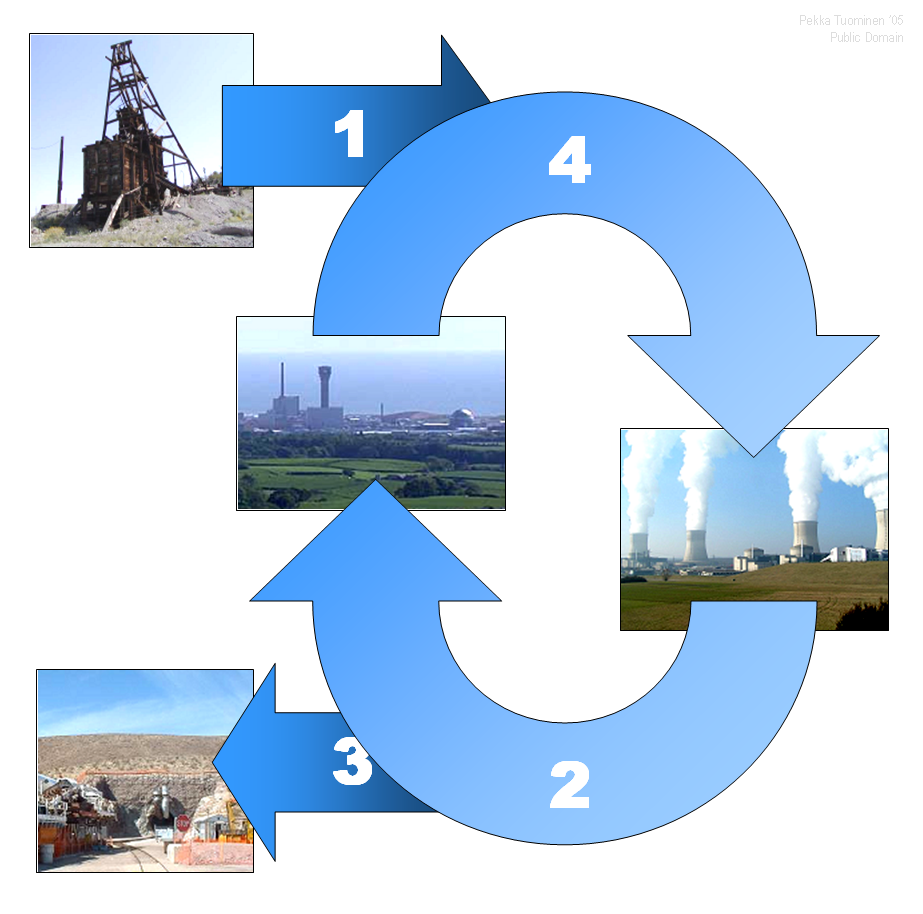
\includegraphics[scale=0.175]{figs/Nuclear_Fuel_Cycle.eps}
\end{center}
\end{slide}


% Motivation
\overlays{5}{
\begin{slide}{Motivation}
\FromSlide{1}
\begin{itemize}
    \item Many nuclear fuel cycle simulations are formulated on premade base-case scenarios:

\FromSlide{2}
    \begin{center}
    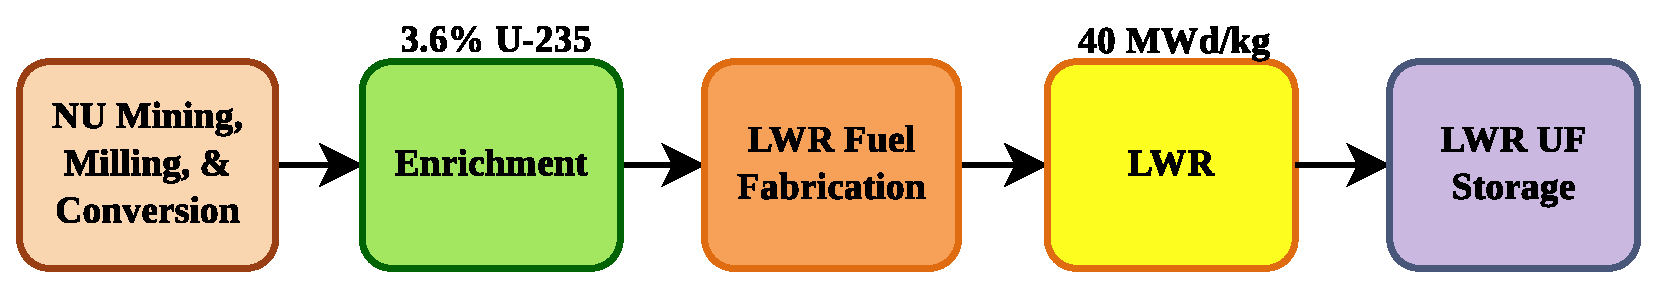
\includegraphics[scale=0.25]{figs/OnceThrough.eps}
    \end{center}

\FromSlide{3}
    \item These base cases are very well studied.

\FromSlide{4}
    \item However, what is \textbf{\textit{not}} well known is 
        how these sample scenarios are affected by perturbations to their 
        initial physical parameters.
            
\FromSlide{1}
\end{itemize}

\FromSlide{5}
\begin{center}
``\textit{Do our parameter choices really give us the `best' solution?}''
\end{center}

\end{slide}}





% Motivation
\begin{slide}{Motivation}
\begin{center}
\begin{figure}
\caption{Physics Modeled versus Execution Time}
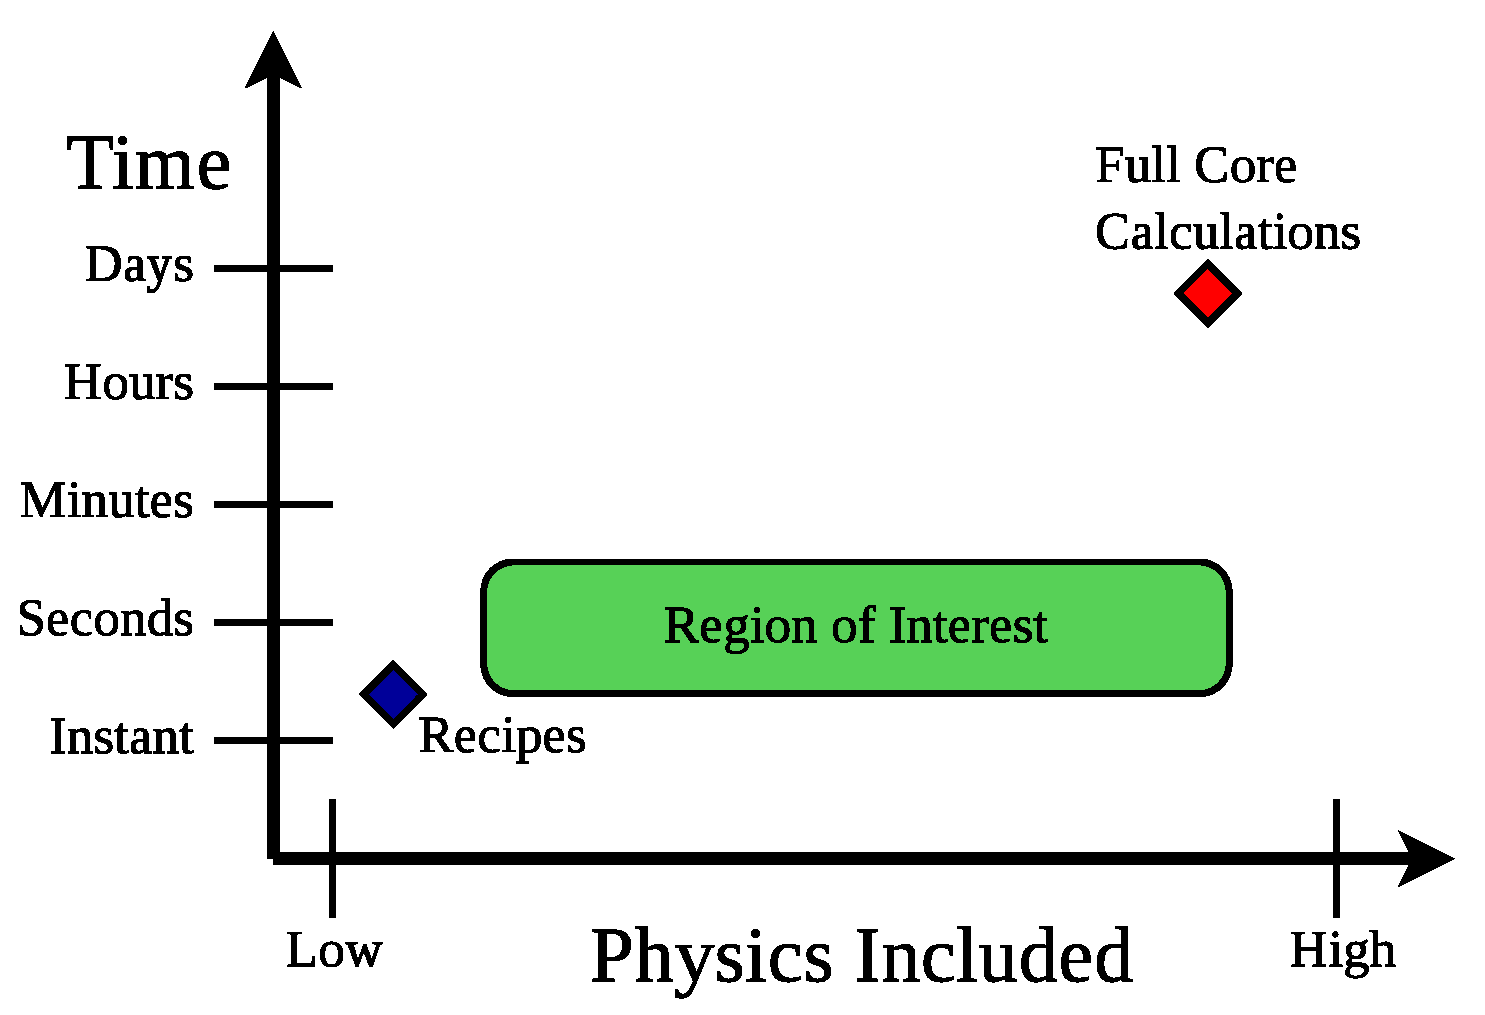
\includegraphics[scale=0.35]{figs/physics_vs_exec_time.eps}
\end{figure}
\end{center}
\end{slide}




% Motivation
\begin{slide}{Motivation}
\small \underline{Basic Fuel Cycle Schema:}
\begin{center}
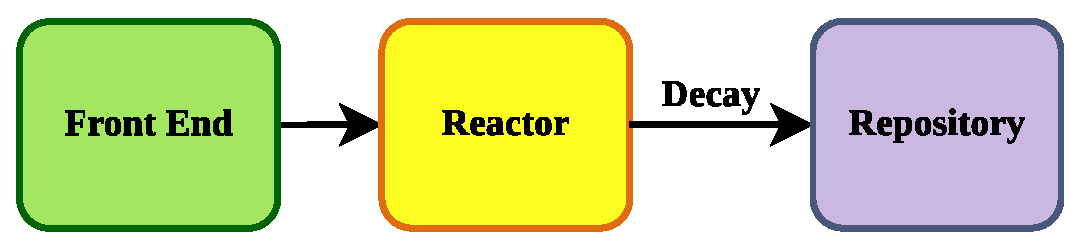
\includegraphics[scale=0.5]{figs/basic_nfc_schema.eps}
\end{center}

\underline{Modeling Approaches:} \small
\begin{center}
\begin{tabular}{lccc}
\textit{Component}                  & \textit{Recipes}  & \textit{Essential} & \textit{Transport}   \\
\underline{\textbf{Front End:}}     & Recipes           & Physics Models     & Physics Models       \\
\underline{\textbf{Reactor:}}       & Recipes           & Rapid Burnup Code  & Neutron Transport    \\
\underline{\textbf{Repository:}}    & Curve Fits        & Rapid Code         & Neutron Transport    \\
\end{tabular}
\end{center}
\end{slide}





% Motivation
\overlays{2}{
\begin{slide}{Motivation}
\FromSlide{1}
\begin{itemize}
    \item Investigating the region of interest may provide a 
        \textit{transformative} amount of fuel cycle data.  

\FromSlide{2}
    \item However, this requires an entirely new spectrum of tools.

\FromSlide{1}
\end{itemize}


\FromSlide{2}
\setcounter{figure}{1}
\begin{center}
\begin{figure}
\caption{Fuel Cycle Stack}
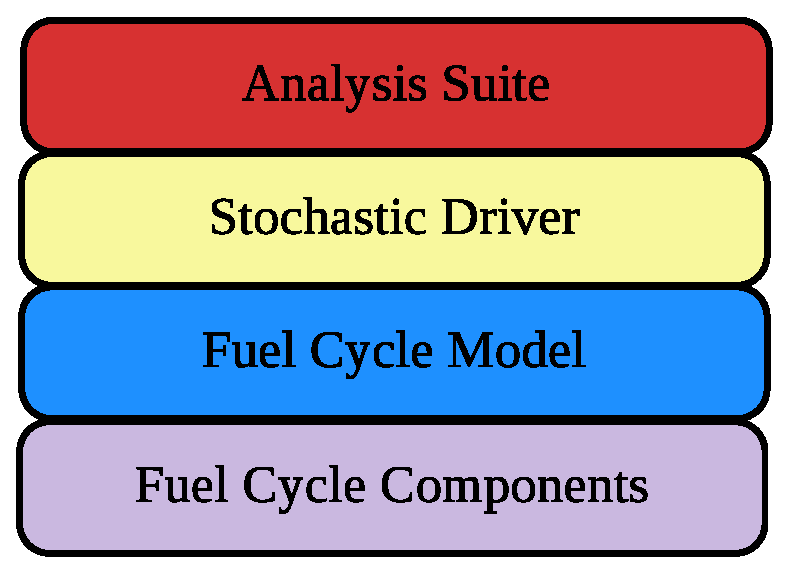
\includegraphics[scale=0.35]{figs/fc_stack.eps}
\end{figure}
\end{center}

\end{slide}}



% Definition
\begin{slide}{Definition}
\vspace{3.0cm}
\begin{center}
\textit{Essential physics} models remain physically valid under perturbations
in the locality of the region that they are defined and do not compute
extraneous parameters.  
\end{center}
\end{slide}




% A Path Forward
\overlays{3}{
\begin{slide}{A Path Forward}
\FromSlide{1}
\begin{itemize}
    \item Develop a set of fuel cycle component models which 
        preserve basic physics (largely focused on one- and 
        multi-energy group reactor models, R1G \& RMG).

\FromSlide{2}
    \item Investigate a categorical set of fuels cycles using
        the above components. These are largely linear 
        perturbations of previous base-case studies. (Skipped
        here in the interest of time.)

\FromSlide{3}
    \item Extend the fuel cycle model to perturb continuous 
        variables.  This requires a stochastic driving mechanism
        to run.  Moreover, it requires entropy-based measures to
        analyze.

\FromSlide{1}
\end{itemize}
\end{slide}}




% R1G \& RMG
\begin{slide}{R1G \& RMG}
\vspace{3.5cm}
\begin{center}
\Large
One- \& Multi-Group Reactor Model
\end{center}
\end{slide}






% R1G
\begin{slide}{R1G}
\begin{center}
\begin{figure}
\caption{Reactor Model [1]}
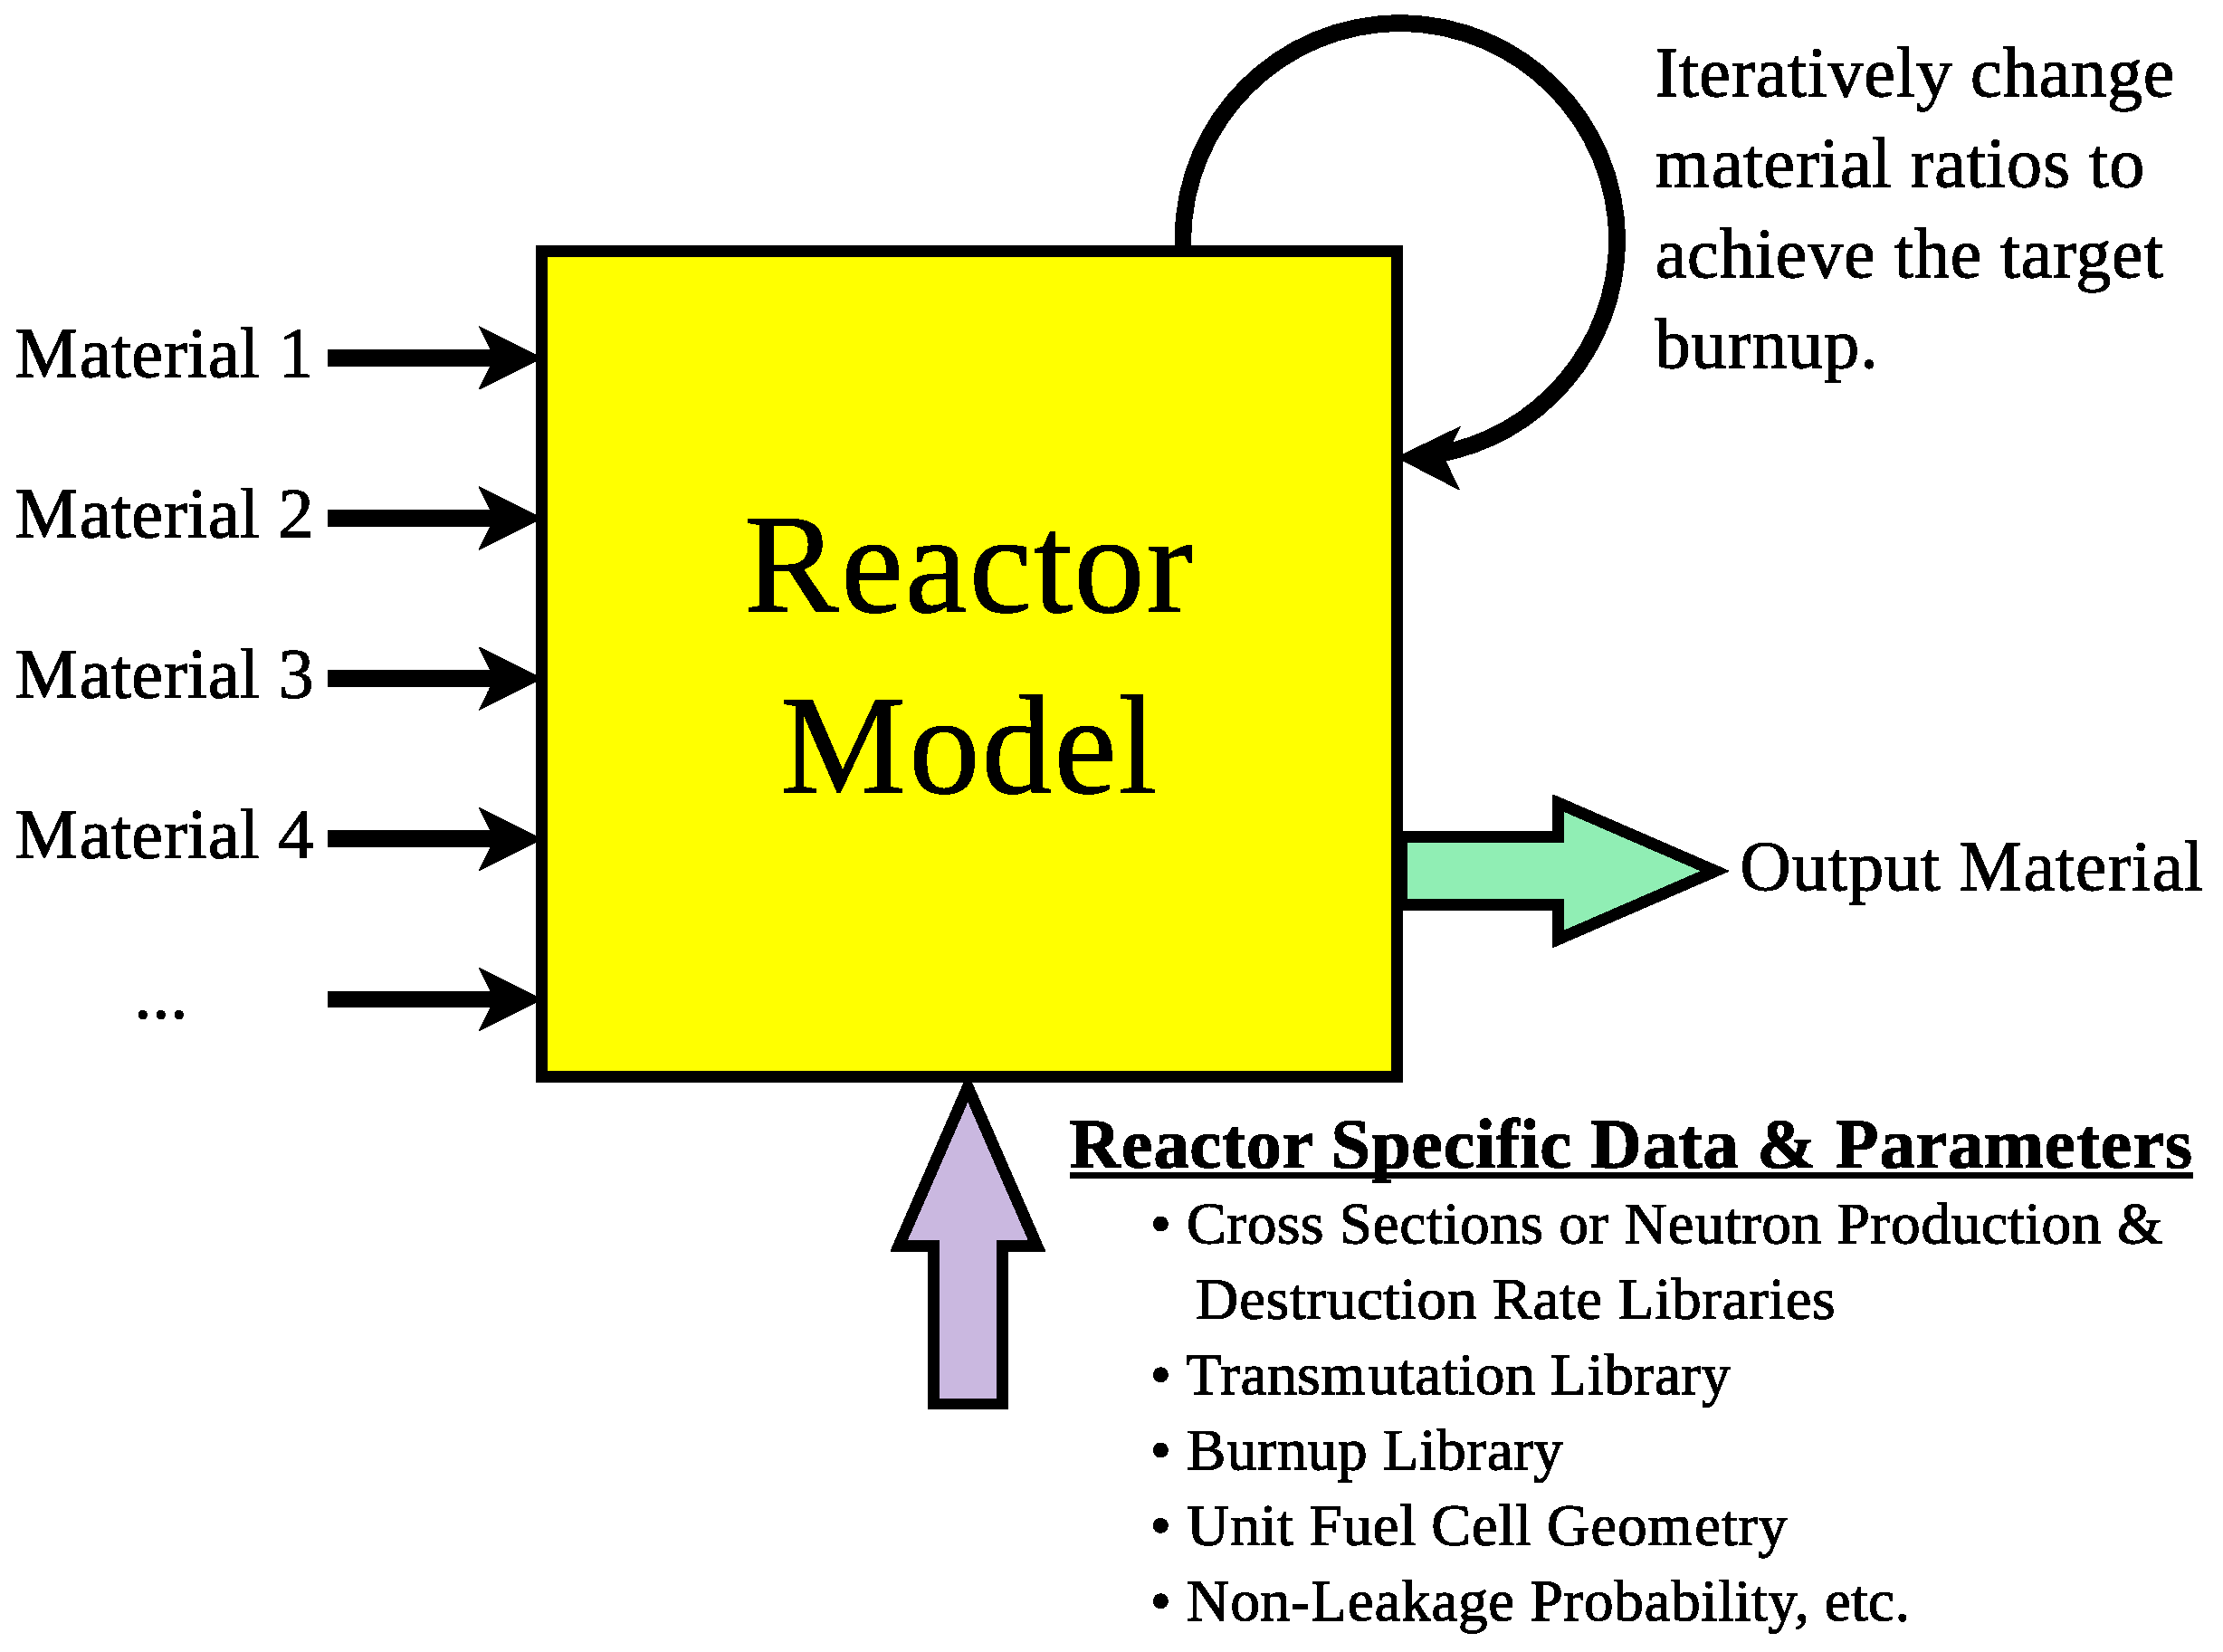
\includegraphics[scale=0.20]{figs/reactor_model.eps}
\end{figure}
\end{center}
\end{slide}




% R1G
\begin{slide}{R1G}
\FromSlide{1}
\begin{center}
Starting with ORIGEN generated fluence-dependent, nuclide specific data, we know:

\setcounter{figure}{3}
\begin{figure}
\subfloat[prod \& des rates,]{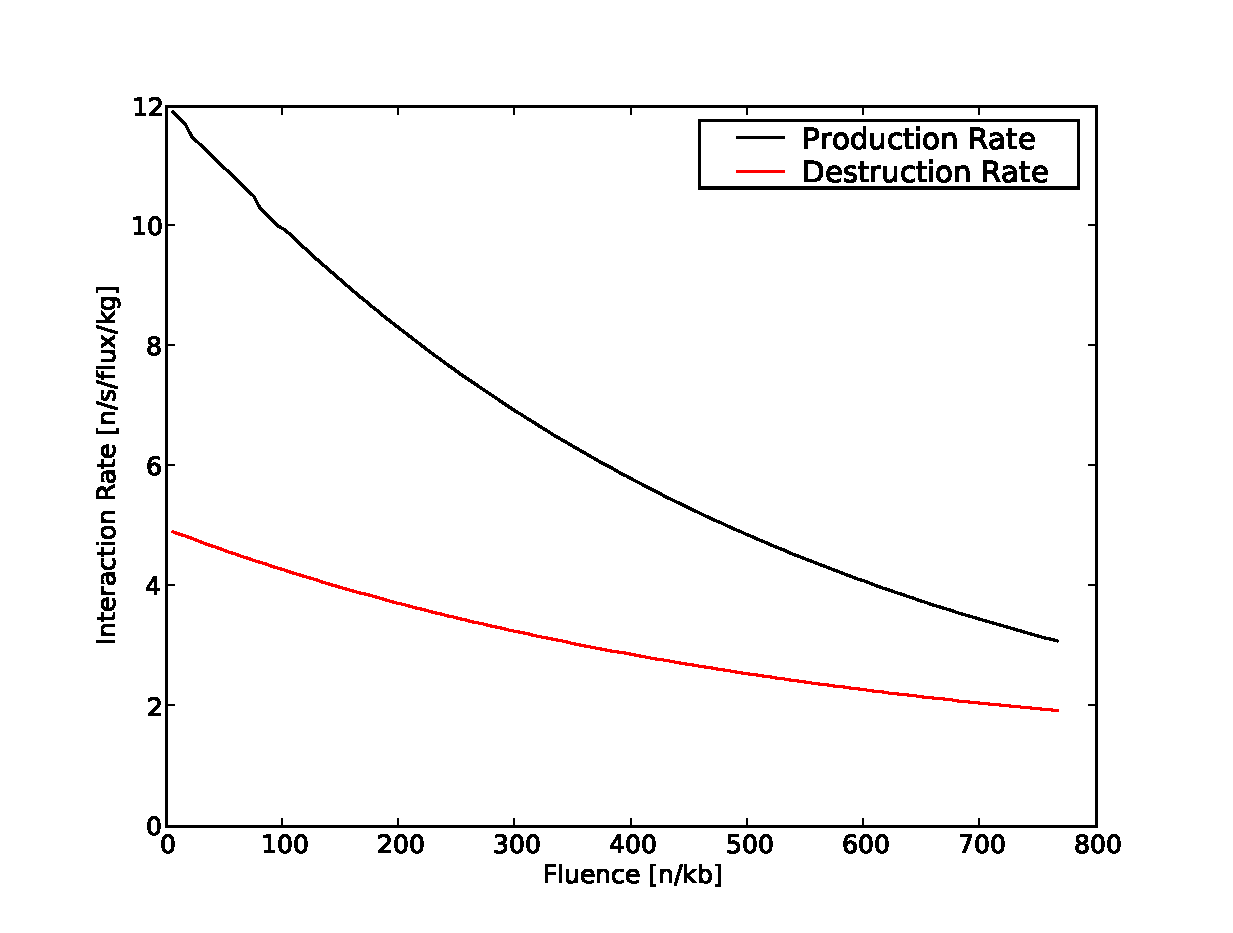
\includegraphics[scale=0.21]{../one_group_method/figs/Fig02.eps}}
\subfloat[burnups,]{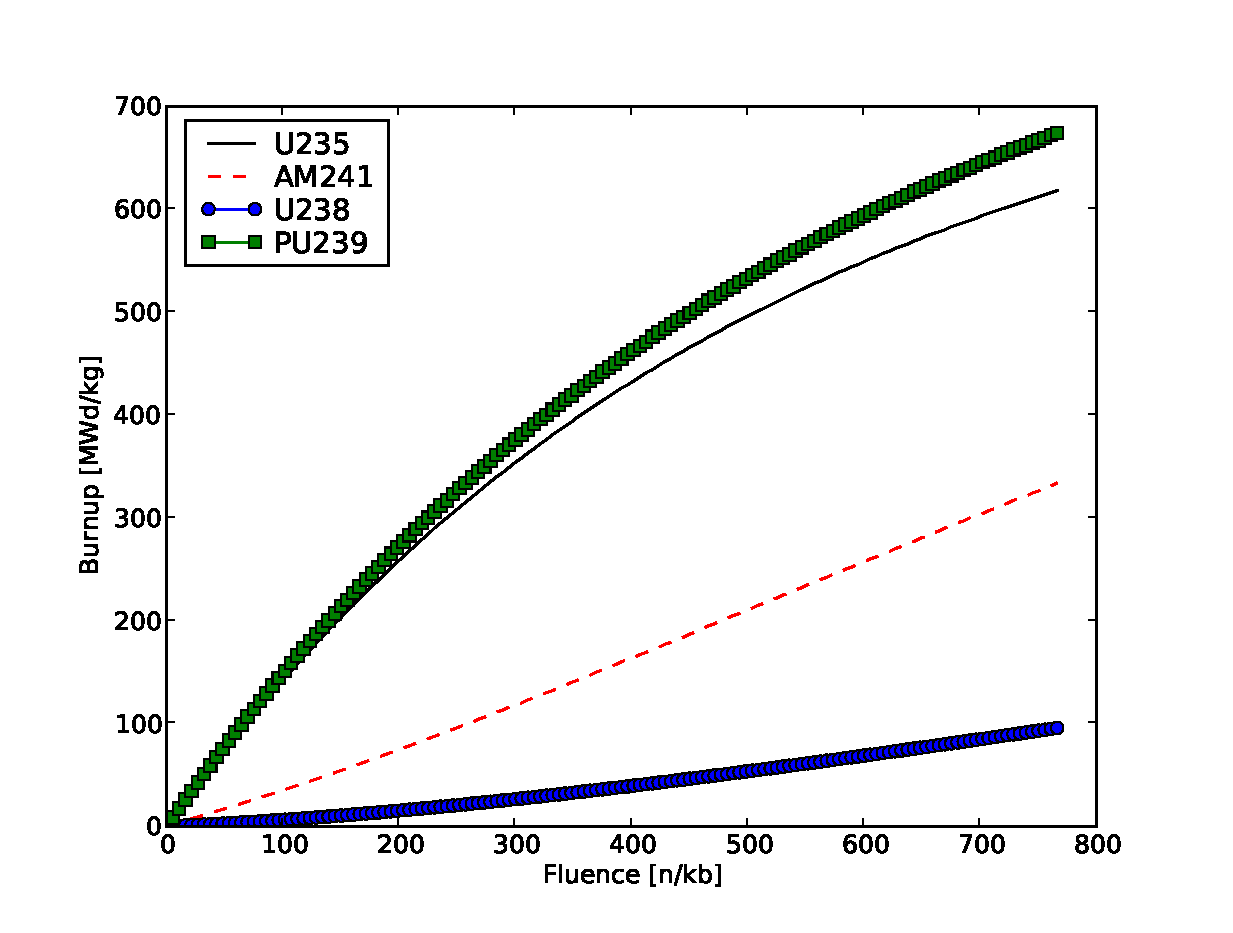
\includegraphics[scale=0.21]{../one_group_method/figs/Fig03.eps}}
\subfloat[transmutation matrices.]{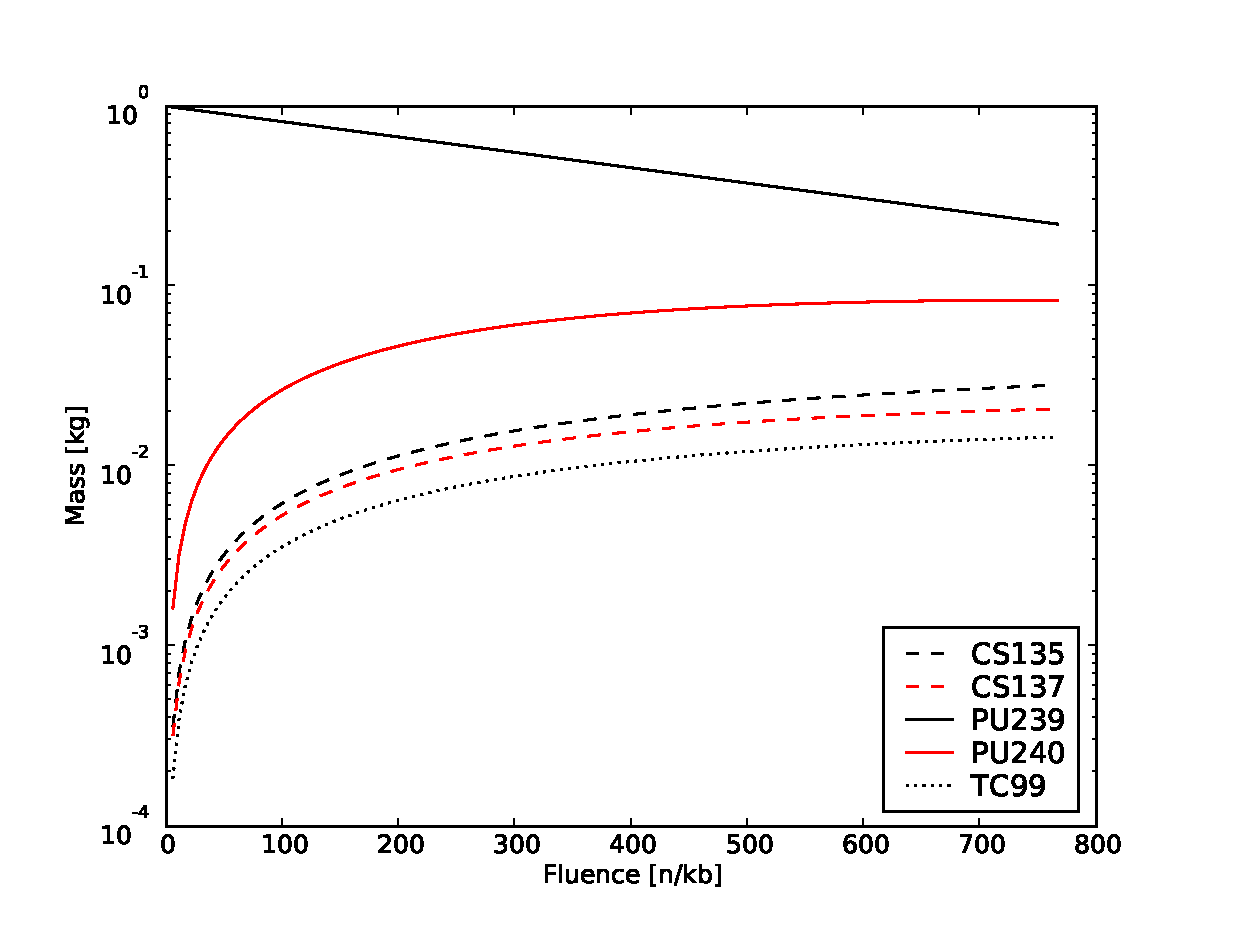
\includegraphics[scale=0.21]{../one_group_method/figs/Fig01.eps}}
\caption{Reactor Data Library (for FR \nuc{Pu}{239})}
\end{figure}

\end{center}
\end{slide}





% R1G
\begin{slide}{R1G}
\begin{center}
\begin{figure}
\caption{Linearly Weighted Fast Reactor Data}
\subfloat[Burnup]{\includegraphics[scale=0.31]{../one_group_method/figs/Fig05.eps}}
\subfloat[Multiplication Factor]{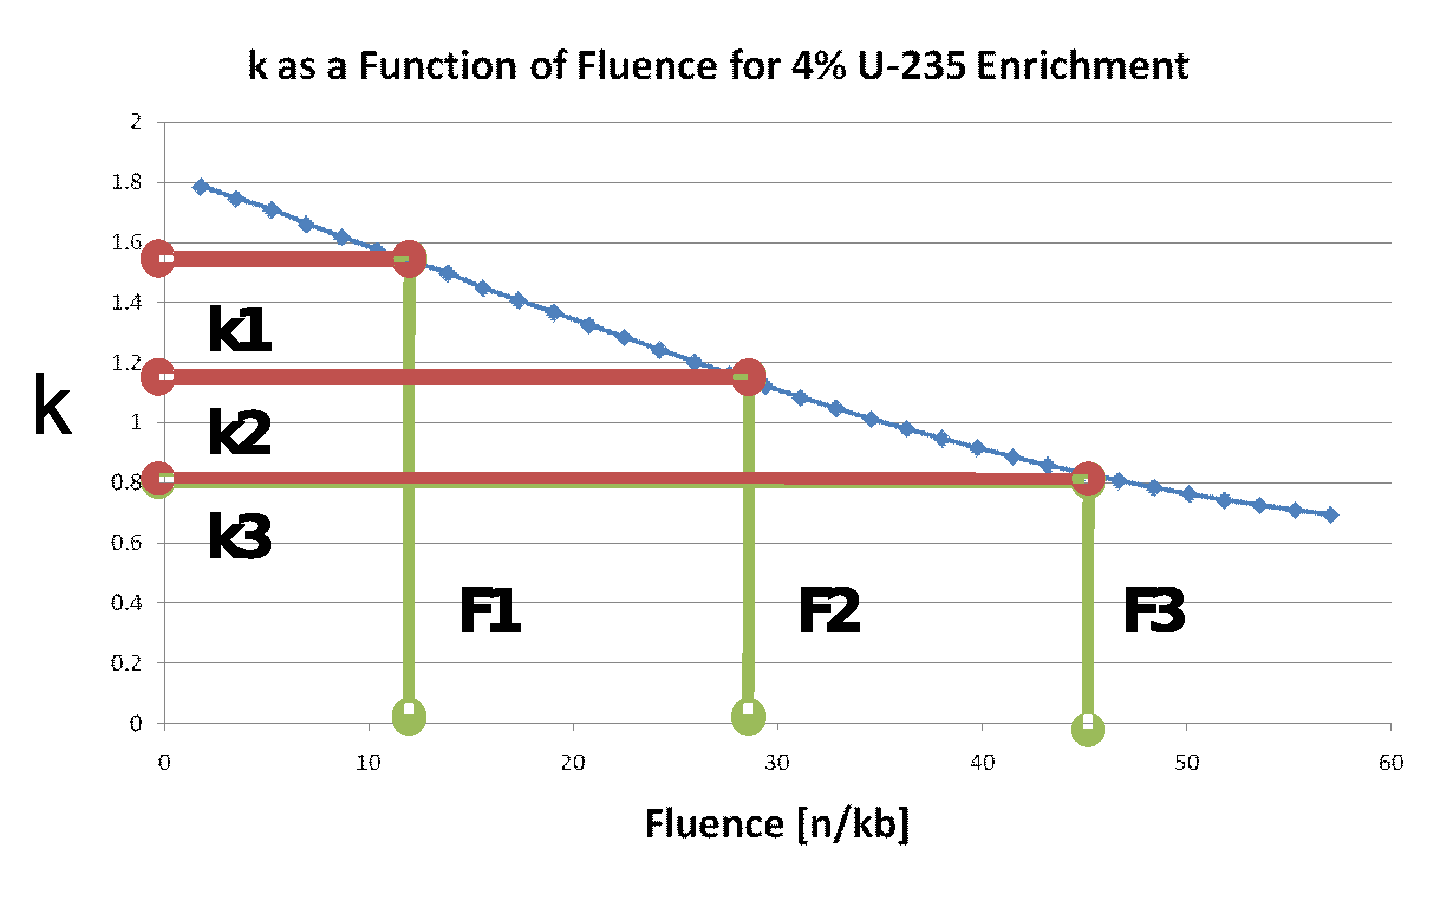
\includegraphics[scale=0.31]{../one_group_method/figs/Fig06.eps}}
\end{figure}
\end{center}
\end{slide}




% R1G 
\overlays{3}{
\begin{slide}{R1G}
\FromSlide{1}
\begin{minipage}[t]{0.49\textwidth}
\setcounter{figure}{5}
\begin{center}
\begin{figure}
\caption{Fast Reactor\\ Discharge Composition}
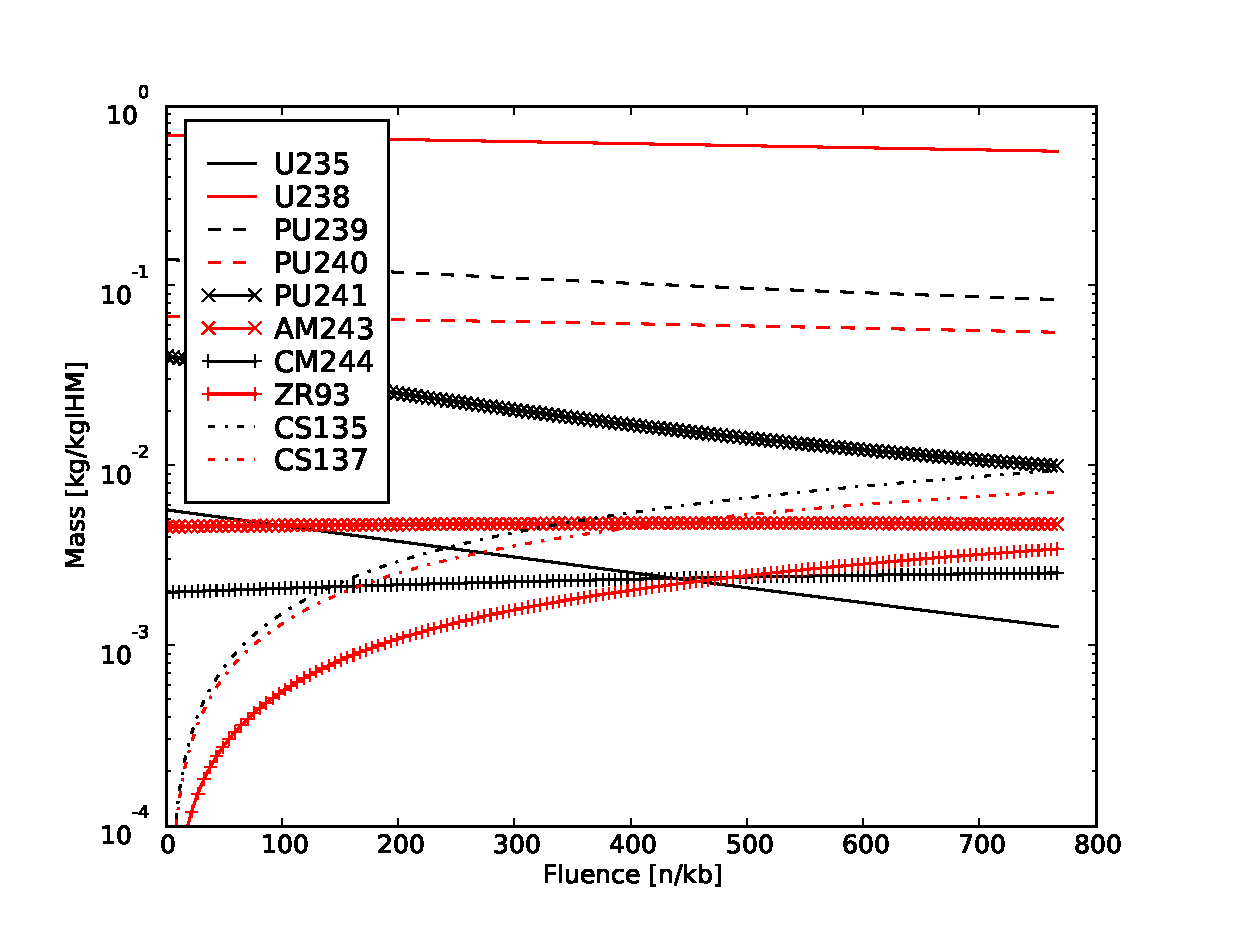
\includegraphics[scale=0.3]{../one_group_method/figs/Fig07.eps}
\end{figure}
\end{center}
\end{minipage}
\begin{minipage}[t]{0.49\textwidth}
\small
\begin{itemize}
    \item The transmutation matrices may be similarly weighted by initial composition.

\FromSlide{2}
    \item From the criticality calculation above we also know the discharge fluence, Fd [n/kb].

\FromSlide{3}
    \item Therefore the used fuel composition is known by taking the nuclide mass weights at 
            Fd in Figure 6.

\FromSlide{1}
\end{itemize}
\end{minipage}
\end{slide}}




% R1G Benchmark
\begin{slide}{R1G Benchmark}
\tiny
\begin{table}[htbp]
\begin{center}
\caption{LWR Benchmark to OECD Burnup Credit [2]}
\begin{tabular}{|l|c|c|c|c|}
\hline
\textbf{Nuclide} & \textbf{OECD [2] [w/o]} & \textbf{$\sigma$ of OECD [\%]} & \textbf{Results [w/o]} & \textbf{\% Difference} \\
\hline
\nuc{U}{234}     & 0.0178  & 9.0  & 0.0184  & +3.6  \\
\nuc{U}{235}     & 0.8001  & 8.1  & 0.7079  & -11.5 \\
\nuc{U}{236}     & 0.4840  & 2.6  & 0.4781  & -1.2  \\
\nuc{U}{238}     & 93.3333 & 0.2  & 93.6109 & +0.3  \\
\nuc{Np}{237}    & 0.0614  & 9.4  & 0.0584  & -5.0  \\
\nuc{Pu}{238}    & 0.0226  & 13.9 & 0.0185  & -18.1 \\
\nuc{Pu}{239}    & 0.5991  & 7.1  & 0.5104  & +14.8 \\
\nuc{Pu}{240}    & 0.2389  & 5.3  & 0.2591  & +8.5  \\
\nuc{Pu}{241}    & 0.1636  & 6.9  & 0.1445  & -11.7 \\
\nuc{Pu}{242}    & 0.0602  & 8.4  & 0.0563  & -6.5  \\
\nuc{Am}{241}    & 0.0047  & 5.3  & 0.0032  & -30.8 \\
\nuc{Am}{243}    & 0.0148  & 10.4 & 0.0116  & -21.3 \\
\hline
\end{tabular}
\end{center}
\end{table}
\end{slide}








% Multi-Group Remotivation
\overlays{3}{
\begin{slide}{Multi-Group Remotivation}
\FromSlide{1}
\begin{itemize}
    \item In the R1G, fluxes are assumed to be static over the course of the burn.

    \FromSlide{2}
    \vspace{1cm}
    \begin{itemize}
        \item This restricts the types of reactors and fuel cycles which may be modeled.
            (MOX, IMF, Traveling Wave, \emph{etc.} are unavailable to the R1G.)
    \end{itemize}

\FromSlide{3}
\vspace{1cm}
    \item Also in the R1G, changing reactor state variables in a way that would affect
        the flux spectrum required additional libraries, or inter-library interpolations.

\FromSlide{1}
\end{itemize}
\end{slide}}





% Remotivation
\overlays{3}{
\begin{slide}{Remotivation}
\FromSlide{1}
\begin{itemize}
    \item To solve these issues, moving to a multi-energy group reactor model 
        will enable automatic spectral shifts in the core as needed.

    \FromSlide{2}
    \vspace{0.75cm}
    \begin{itemize}
        \item Rather than parameterizing burnup, transmutation, and neutron 
            production \& destruction rates as functions of nuclide and fluence, 
            the RMG parameterizes cross sections over a number of different states.
    \end{itemize}

\FromSlide{3}
\vspace{0.75cm}
    \item The R1G parameters are explicitly solved for by the RMG model.

\FromSlide{1}
\end{itemize}
\end{slide}}





% Cross Section Parameterization
\begin{slide}{Cross Section Parameterization}
\begin{itemize}
    \item Group constants are denoted by $\sigma_{r_x,i\tau g}$ or $\sigma_{r_x,ipg}$ [b].
    \item Group-to-group scattering by $\sigma_{s,i\tau g\to h}$ or $\sigma_{s,ipg\to h}$.
\end{itemize}
\begin{table}[htbp]
\begin{center}
\caption{Cross Section Indices}
\label{rmg_xs_ind}
\begin{tabular}{|l|c|}
\hline
\small
\textbf{Index}        & \textbf{Symbol} \\
\hline
Nuclide               & $i$ \\
Time                  & $\tau$ \\
Perturbation          & $p$ \\
Incident Energy Group & $g$ \\
Exiting Energy Group  & $h$ \\
Reaction Channel [5] & $r_x$ \\
\hline
\end{tabular}
\end{center}
\end{table}
\end{slide}



% Reactor State Variables
\begin{slide}{Reactor State Variables}
\begin{table}[htbp]
\begin{center}
\tiny
\caption{Parameters $a_p$ which Define a Perturbation}
\begin{tabular}{|l|c|c|}
\hline
\textbf{Parameter}            & \textbf{Symbol}      & \textbf{Units} \\
\hline
Fuel Density                  & $\rho_{\mbox{fuel}}$ & g/cm\superscript{3}  \\
Cladding Density              & $\rho_{\mbox{clad}}$ & g/cm\superscript{3}  \\
Coolant Density               & $\rho_{\mbox{cool}}$ & g/cm\superscript{3}  \\
Fuel Cell Radius              & $r_{\mbox{fuel}}$    & cm \\
Void Cell Radius              & $r_{\mbox{void}}$    & cm \\
Cladding Cell Radius          & $r_{\mbox{clad}}$    & cm \\
Unit Cell Pitch               & $\ell$               & cm \\
Number of Burn Regions        & $b_r$                &  \\
Fuel Specific Power           & $p_s$                & MW/kgIHM \\
Initial Nuclide Mass Fraction & $T_{i0}$             & kg\subscript{i}/kgIHM \\
Burn Times                    & $s$                  & days \\
\hline
\end{tabular}
\end{center}
\end{table}
\end{slide}





% Reactor State Variables
\begin{slide}{Reactor State Variables}
\begin{table}[htbp]
\begin{center}
\caption{Outer Product Perturbations}
\tiny
\begin{tabular}{|ccccccccccc|}
\hline
\textbf{$\rho_{\mbox{fuel}}$} & \textbf{$\rho_{\mbox{clad}}$} & \textbf{$\rho_{\mbox{cool}}$} & \textbf{$r_{\mbox{fuel}}$} & \textbf{$r_{\mbox{void}}$} & \textbf{$r_{\mbox{clad}}$} & \textbf{$\ell$} & \textbf{$b_r$} & \textbf{$p_s$} & \textbf{$T_{\mbox{\nuc{U}{235}0}}$} & \textbf{$s$} \\
\hline
10.165 & 5.87 & 0.73 & 0.41 & 0.4185 & 0.475 & 1.3127 & 10 & 0.04 & 0.03 & 0   \\
10.165 & 5.87 & 0.73 & 0.41 & 0.4185 & 0.475 & 1.3127 & 10 & 0.04 & 0.03 & 100 \\
10.165 & 5.87 & 0.73 & 0.41 & 0.4185 & 0.475 & 1.3127 & 10 & 0.04 & 0.03 & 200 \\
10.165 & 5.87 & 0.73 & 0.41 & 0.4185 & 0.475 & 1.3127 & 10 & 0.04 & 0.03 & 300 \\
10.165 & 5.87 & 0.73 & 0.41 & 0.4185 & 0.475 & 1.3127 & 10 & 0.04 & 0.03 & 400 \\
10.165 & 5.87 & 0.73 & 0.41 & 0.4185 & 0.475 & 1.3127 & 10 & 0.04 & 0.05 & 0   \\
10.165 & 5.87 & 0.73 & 0.41 & 0.4185 & 0.475 & 1.3127 & 10 & 0.04 & 0.05 & 100 \\
10.165 & 5.87 & 0.73 & 0.41 & 0.4185 & 0.475 & 1.3127 & 10 & 0.04 & 0.05 & 200 \\
10.165 & 5.87 & 0.73 & 0.41 & 0.4185 & 0.475 & 1.3127 & 10 & 0.04 & 0.05 & 200 \\
10.165 & 5.87 & 0.73 & 0.41 & 0.4185 & 0.475 & 1.3127 & 10 & 0.04 & 0.05 & 300 \\
10.165 & 5.87 & 0.73 & 0.41 & 0.4185 & 0.475 & 1.3127 & 10 & 0.04 & 0.05 & 400 \\
$\vdots$ & $\vdots$ & $\vdots$ & $\vdots$ & $\vdots$ & $\vdots$ & $\vdots$ & $\vdots$ & $\vdots$ & $\vdots$ & $\vdots$ \\
\hline
\end{tabular}
\end{center}
\end{table}
\end{slide}









% RMG Methodology
% Getting this figure was tricky
%   1. Modified version of method_diagram.tex put in figs/ (added document info)
%   2. Ran latex on this file to get dvi
%   3. Rand dvips to get post-script file.
% Oddly this was easier than try to change the fonts inside of the figure file
\begin{slide}{RMG Methodology}
\begin{center}
\begin{figure}
\caption{Multigroup Reactor Model Flow Diagram}
\includegraphics[scale=0.45, clip, trim=1.5cm 6.75cm 1.5cm 6.75cm]{figs/method_diagram.ps}
\end{figure}
\end{center}
\end{slide}




% RMG Metric Space
\overlays{3}{
\begin{slide}{RMG Metric Space}
\FromSlide{1}
\begin{itemize}
    \item With $p$ as the perturbation index ($1 \le p \le n_p$),
        $a_p$ is a parameter value in the library and $a_r$ the value on the 
        reactor at run time.

\FromSlide{2}
    \item The distance from any perturbation to the current reactor is given 
        by $d_p$:

        \[ d_p = \sqrt{\sum_a \left(\frac{a_r - a_p}{a_{n_p}}\right)^2} \]

\FromSlide{3}
    \item The sequence $p^*$ determines the nearest neighbors:

        \[ p^* = \left\{p | d_p \le d_{p+1}\right\} \]

\FromSlide{1}
\end{itemize}
\end{slide}}






% Cross Section Interpolation
\overlays{3}{
\begin{slide}{Cross Section Interpolation}
\FromSlide{1}
\begin{itemize}
    \item Using the shorthand $a_p^*$ as a substitute for $a_{p^*}$, 

\FromSlide{2}
    \vspace{0.5cm}
    \item Then $x_f$ is a unitless multidimensional linear interpolation factor,

        \[ x_f = \sum_a \left(\frac{a_r - a_1^*}{a_2^* - a_1^*}\right) \]

\FromSlide{3}
    \vspace{0.5cm}
    \item Group constants \textit{for each time step} are computed:

        \[ \sigma_{r_x,i\tau g} = (\sigma_{r_x,ip_2^*g} - \sigma_{r_x,ip_1^*g}) \cdot x_f  + \sigma_{r_x,ip_1^*g} \]

\FromSlide{1}
\end{itemize}
\end{slide}}



% Criticality Calculation
\overlays{3}{
\begin{slide}{Criticality Calculation}
\scriptsize
\FromSlide{1}
\begin{itemize}
    \item The shape of the spectrum is given by an iterative solution to a matrix method.

        \[ A_{\tau g\to h} \cdot \phi_{\tau g} = \frac{1}{k} F_{\tau g\to h} \cdot \phi_{\tau g} \]

\FromSlide{2}
    \item ...with a rescaling to obtain the magnitude, 

        \[ \phi_{\tau} = p_s \cdot  \rho_{\mbox{fuel}} \cdot \frac{1}
                                                                  {\mbox{3.284E-14} \cdot \Sigma_{f,\mbox{fuel},\tau}} \]

\FromSlide{3}
    \item and a side calculation to obtain the multiplication factor.

        \[ k_{\tau} = P_{\mbox{NL}} \cdot \frac{\sum_g^G V_{\mbox{fuel}} \cdot \bar{\nu}\Sigma_{f,\mbox{fuel},\tau g} \cdot \phi_{\tau g}}
                                               {\sum_g^G \left(V_{\mbox{fuel}} \cdot \Sigma_{a,\mbox{fuel},\tau g} + \zeta_{\tau g} \cdot V_{\mbox{cool}} \cdot \Sigma_{a,\mbox{cool},\tau g}\right) \cdot  \phi_{\tau g}}  \]

\FromSlide{1}
\end{itemize}
\end{slide}}





% Transmutation Calculation
\overlays{2}{
\begin{slide}{Transmutation Calculation}
\FromSlide{1}
\begin{itemize}
    \item ORIGEN 2.2 [7] is used as the transmutation kernel for the RMG.

\FromSlide{2}
    \vspace{1cm}
    \item Custom ORIGEN cross section libraries are built for each time step.  
        The group constants for the current reactor state are simply collapsed.

        \[ \sigma_{r_x,i\tau} = \frac{1}{\phi_{\tau}} \sum_g^G \sigma_{r_x,i\tau g} \phi_{\tau g} \]

\FromSlide{1}
\end{itemize}
\end{slide}}






% RMG Benchmark
\overlays{2}{
\begin{slide}{RMG Benchmark}
\FromSlide{1}
\begin{itemize}
    \item The RMG was benchmarked against a Serpent run where both transport and essential 
        physics methods were fed the OECD's LWR Burnup Credit reactor [2].  

\FromSlide{2}
    \vspace{1.25cm}
    \item The benchmark examines the first year of the burn with an initial \nuc{U}{235}
        enrichment of 4.5 [w/o].

\FromSlide{1}
\end{itemize}
\end{slide}}





% RMG Benchmark
\begin{slide}{RMG Benchmark}
\begin{table}[htbp]
\begin{center}
\caption{Nearest Neighbors over Burn}
\label{nn_table}
\tiny
\begin{tabular}{|l||cc|ccccccccccccccc|}
\hline
\textbf{days} & \multicolumn{17}{|c|}{\textbf{$p^*$}} \\
\hline
0 & 16 & 6 & 17 & 7 & 18 & 8 & 11 & 1 & 9 & 19 & 12 & 2 & 13 & 3 & 10 & 20 & $\cdots$ \\
40.6 & 16 & 6 & 17 & 7 & 18 & 8 & 19 & 9 & 11 & 1 & 12 & 2 & 13 & 3 & 10 & 20 & $\cdots$ \\ 
81.1 & 17 & 7 & 16 & 6 & 18 & 8 & 19 & 9 & 2 & 12 & 11 & 1 & 13 & 3 & 10 & 20 & $\cdots$ \\
122 & 7 & 17 & 18 & 8 & 6 & 16 & 19 & 9 & 20 & 10 & 2 & 12 & 3 & 13 & 11 & 1 & $\cdots$ \\
162 & 8 & 18 & 7 & 17 & 19 & 9 & 6 & 16 & 20 & 10 & 3 & 13 & 2 & 12 & 4 & 14 & $\cdots$ \\
203 & 18 & 8 & 19 & 9 & 17 & 7 & 10 & 20 & 6 & 16 & 3 & 13 & 4 & 14 & 12 & 2 & $\cdots$ \\
243 & 18 & 8 & 19 & 9 & 17 & 7 & 10 & 20 & 6 & 16 & 3 & 13 & 4 & 14 & 12 & 2 & $\cdots$ \\
284 & 19 & 9 & 18 & 8 & 10 & 20 & 7 & 17 & 4 & 14 & 6 & 16 & 3 & 13 & 5 & 15 & $\cdots$ \\
324 & 19 & 9 & 10 & 20 & 8 & 18 & 7 & 17 & 4 & 14 & 5 & 15 & 3 & 13 & 6 & 16 & $\cdots$ \\
365 & 10 & 20 & 19 & 9 & 18 & 8 & 7 & 17 & 5 & 15 & 4 & 14 & 3 & 13 & 6 & 16 & $\cdots$ \\
\hline
\end{tabular}
\end{center}
\end{table}
\end{slide}





% RMG Benchmark
\begin{slide}{RMG Benchmark}
\begin{center}
\begin{figure}
\caption{Multiplication Factor Benchmark}
\includegraphics[scale=0.4]{../multigroup_method/figs/benchmark/k.eps}
\end{figure}
\end{center}
\end{slide}






% RMG Benchmark
\begin{slide}{RMG Benchmark}
\begin{center}
\begin{figure}
\caption{Neutron Flux Spectrum Benchmarks}
\subfloat[BOL]{\includegraphics[scale=0.3]{../multigroup_method/figs/benchmark/Normalized_Flux_at_0_days.eps}}
\subfloat[EOL]{\includegraphics[scale=0.3]{../multigroup_method/figs/benchmark/Normalized_Flux_at_365_days.eps}}
\end{figure}
\end{center}
\end{slide}




% RMG Benchmark
\begin{slide}{RMG Benchmark}
\vspace{0.75cm}
\begin{center}
\begin{figure}
\caption{Selected Actinide Mass Fractions}
\subfloat[\nuc{U}{235}]{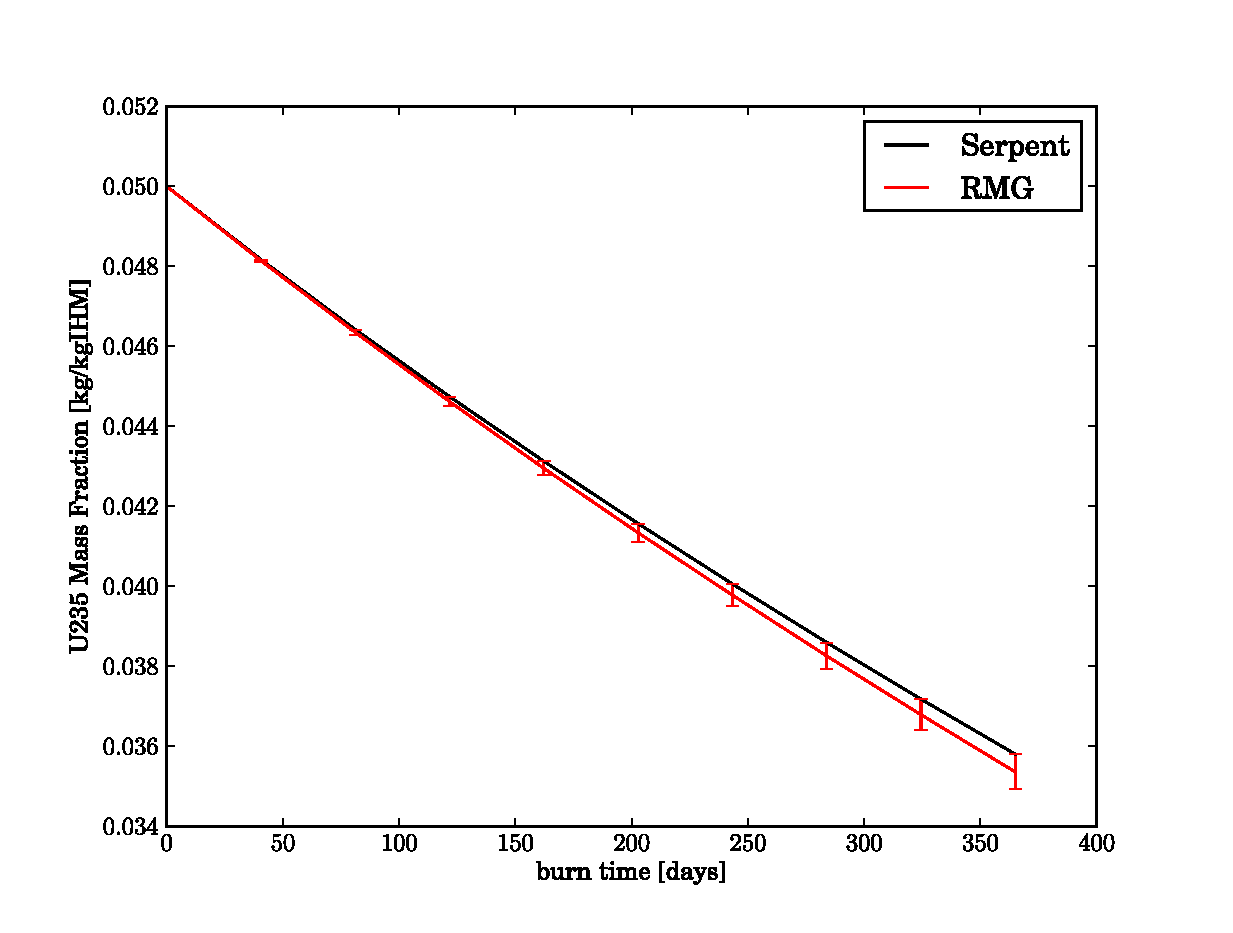
\includegraphics[scale=0.21]{../multigroup_method/figs/benchmark/U235_Mass_Fraction_.eps}}
\subfloat[\nuc{U}{238}]{\includegraphics[scale=0.21]{../multigroup_method/figs/benchmark/U238_Mass_Fraction_.eps}}
\subfloat[\nuc{Pu}{239}]{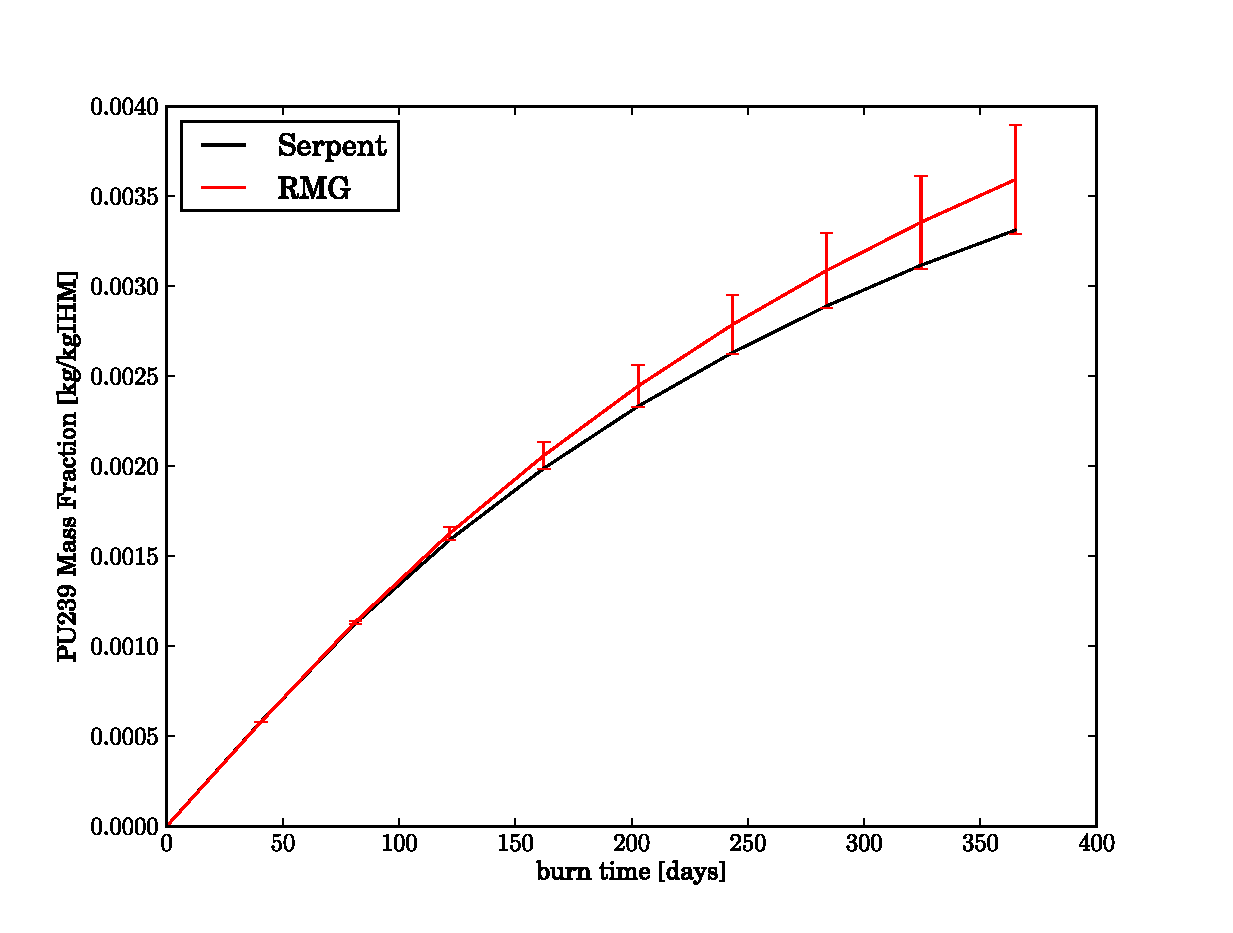
\includegraphics[scale=0.21]{../multigroup_method/figs/benchmark/PU239_Mass_Fraction_.eps}}
\end{figure}
\end{center}
\end{slide}




% RMG Benchmark
\begin{slide}{RMG Benchmark}
\vspace{0.75cm}
\begin{center}
\begin{figure}
\caption{Selected Actinide Mass Fractions}
\subfloat[\nuc{Pu}{240}]{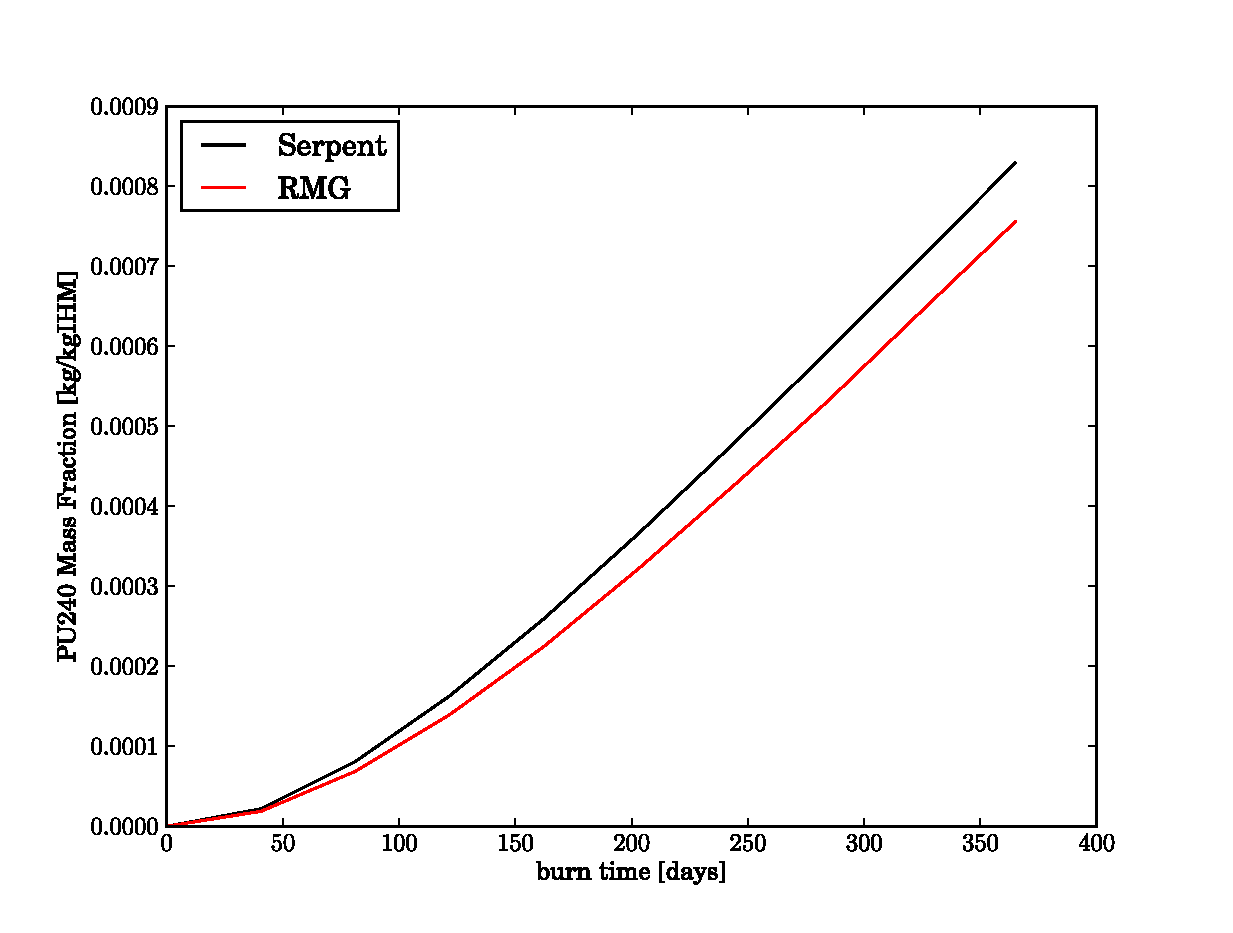
\includegraphics[scale=0.21]{../multigroup_method/figs/benchmark/PU240_Mass_Fraction_.eps}}
\subfloat[\nuc{Am}{242}]{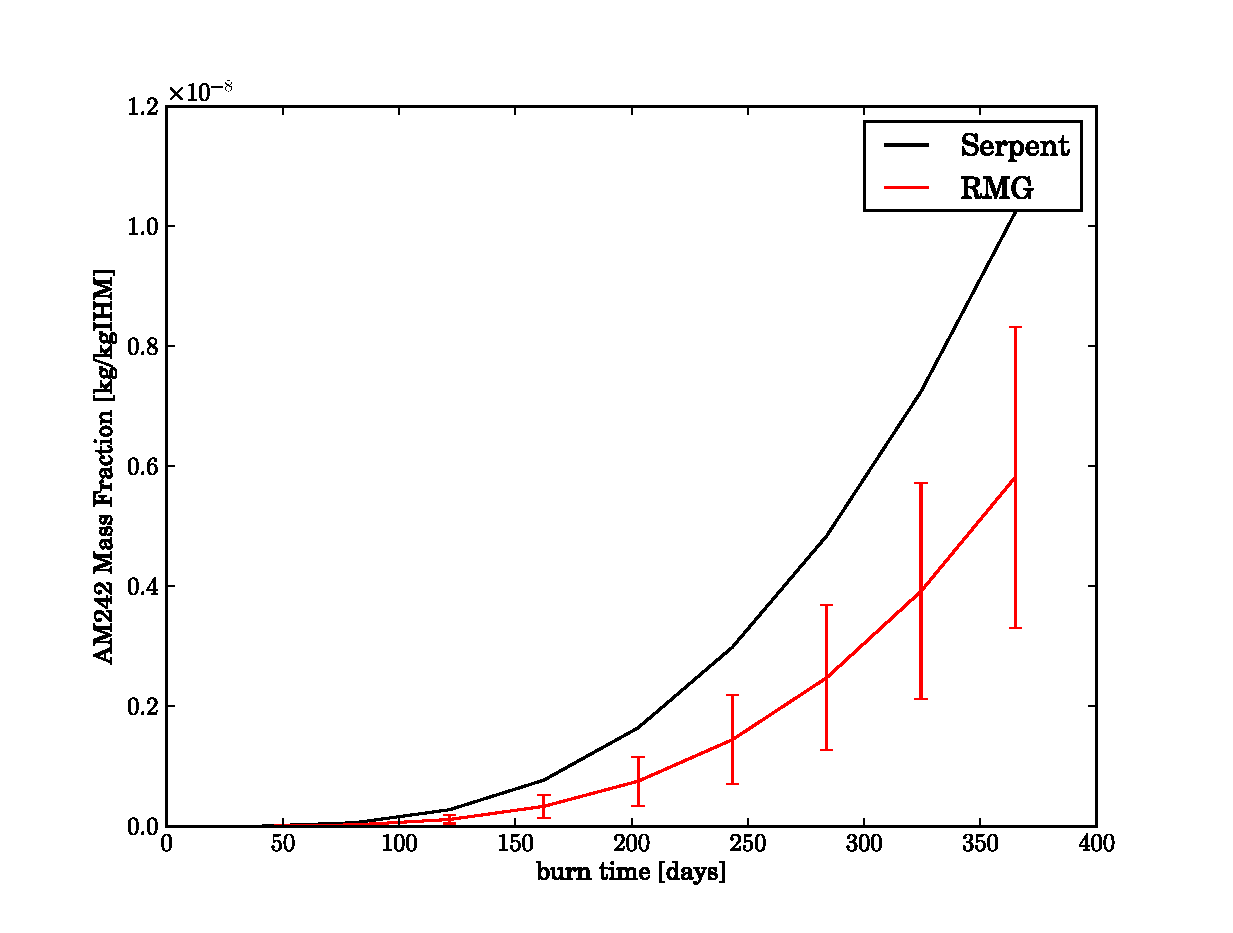
\includegraphics[scale=0.21]{../multigroup_method/figs/benchmark/AM242_Mass_Fraction_.eps}}
\subfloat[\nuc{Cm}{246}]{\includegraphics[scale=0.21]{../multigroup_method/figs/benchmark/CM246_Mass_Fraction_.eps}}
\end{figure}
\end{center}
\end{slide}



% RMG Benchmark
\begin{slide}{RMG Benchmark}
\vspace{0.75cm}
\begin{center}
\begin{figure}
\caption{Selected Fission Product Mass Fractions}
\subfloat[\nuc{Sr}{90}]{\includegraphics[scale=0.21]{../multigroup_method/figs/benchmark/SR90_Mass_Fraction_.eps}}
\subfloat[\nuc{Tc}{99}]{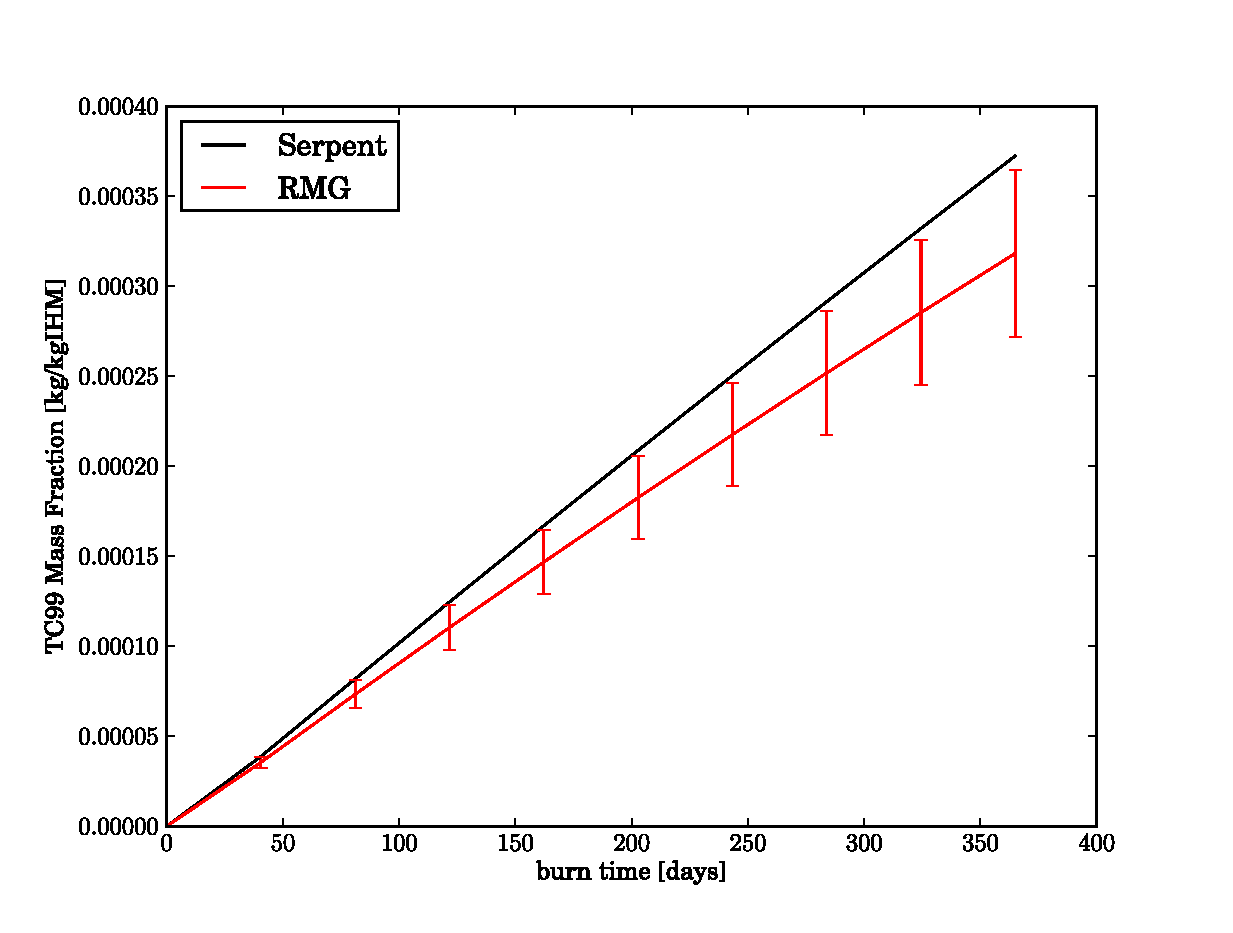
\includegraphics[scale=0.21]{../multigroup_method/figs/benchmark/TC99_Mass_Fraction_.eps}}
\subfloat[\nuc{Cs}{137}]{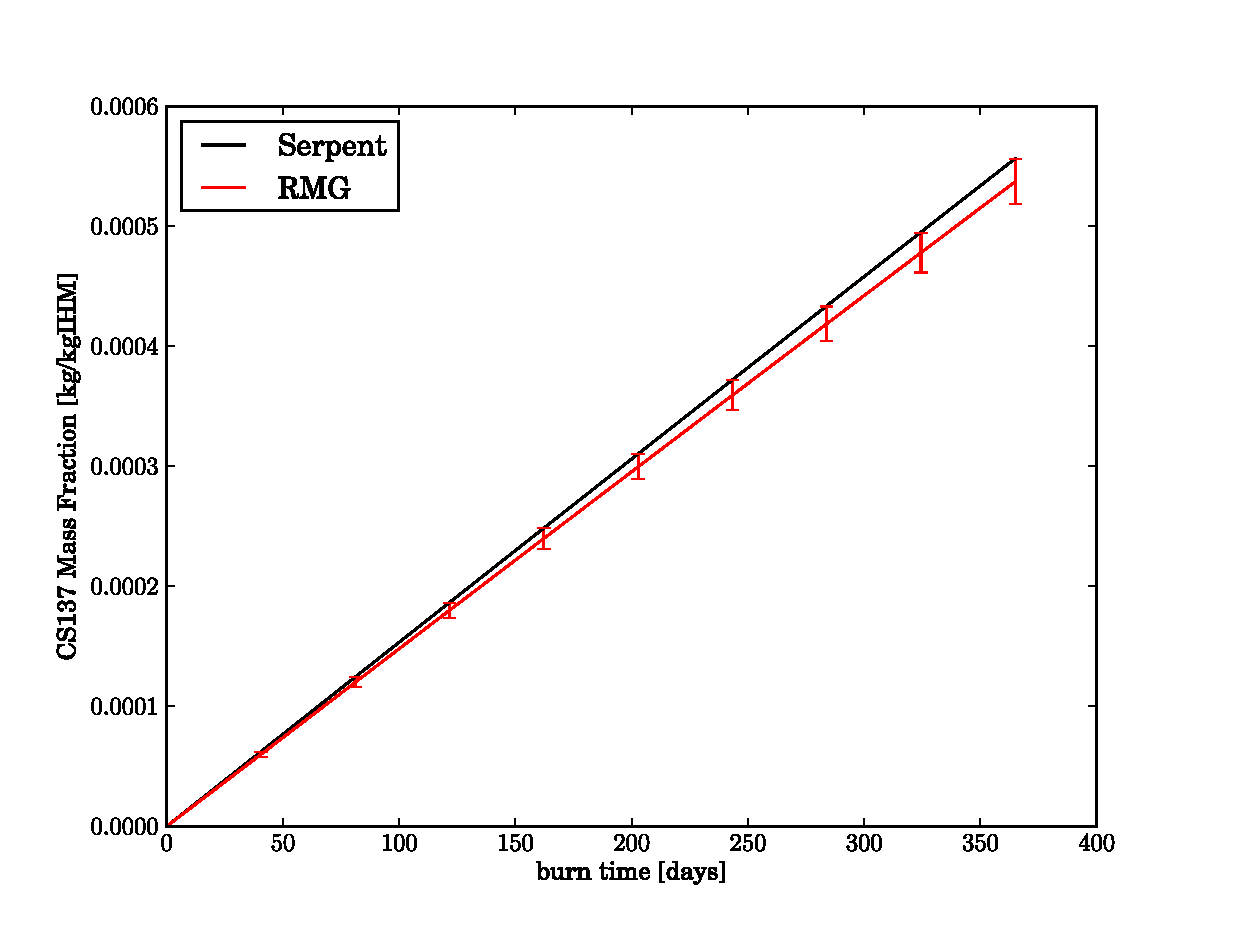
\includegraphics[scale=0.21]{../multigroup_method/figs/benchmark/CS137_Mass_Fraction_.eps}}
\end{figure}
\end{center}
\end{slide}






% RMG Benchmark
\begin{slide}{RMG Benchmark}
\vspace{0.75cm}
\begin{center}
\begin{figure}
\caption{Selected Actinide One-Group Cross-Sections}
\subfloat[\nuc{U}{235}]{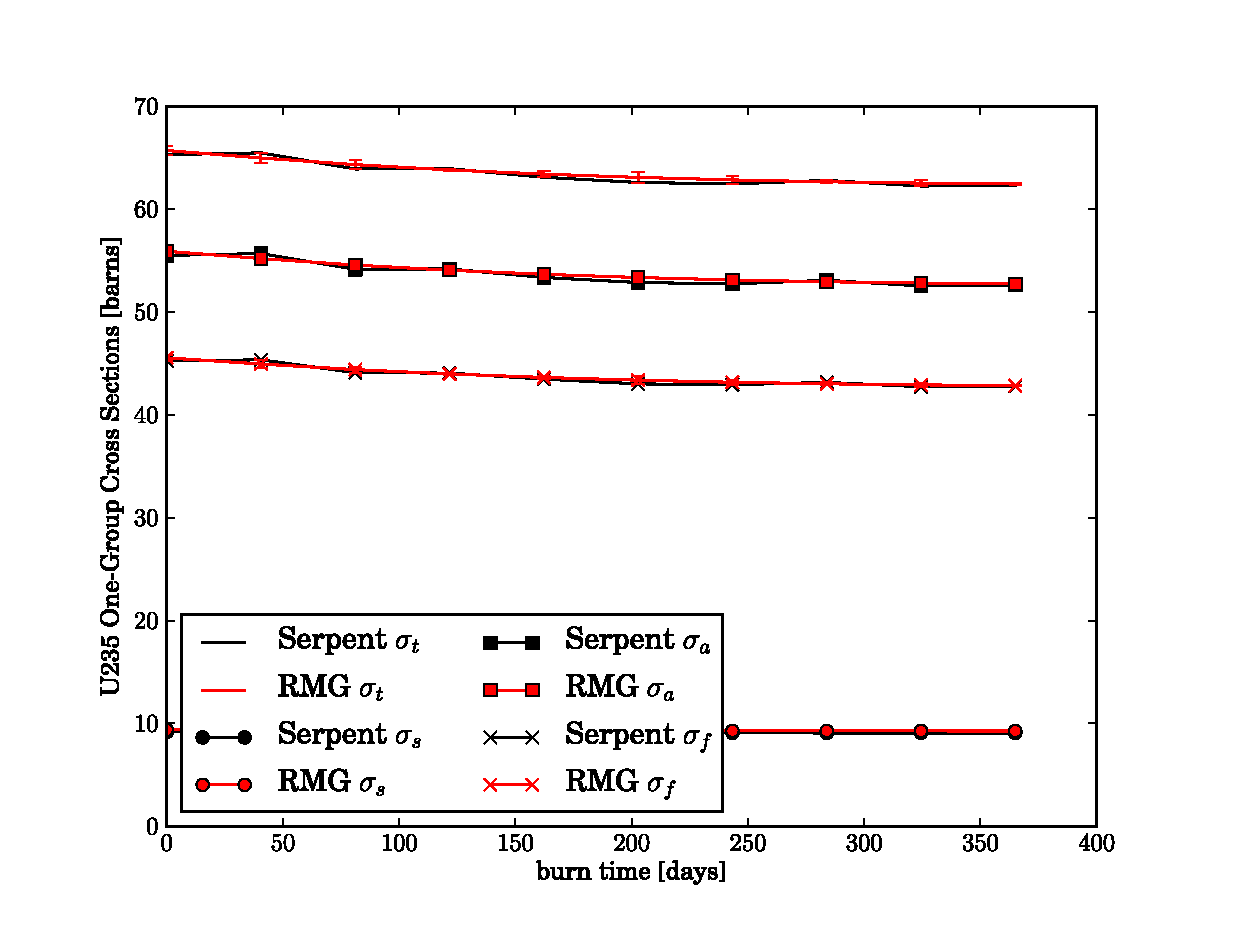
\includegraphics[scale=0.21]{../multigroup_method/figs/benchmark/U235_1g_xs.eps}}
\subfloat[\nuc{U}{238}]{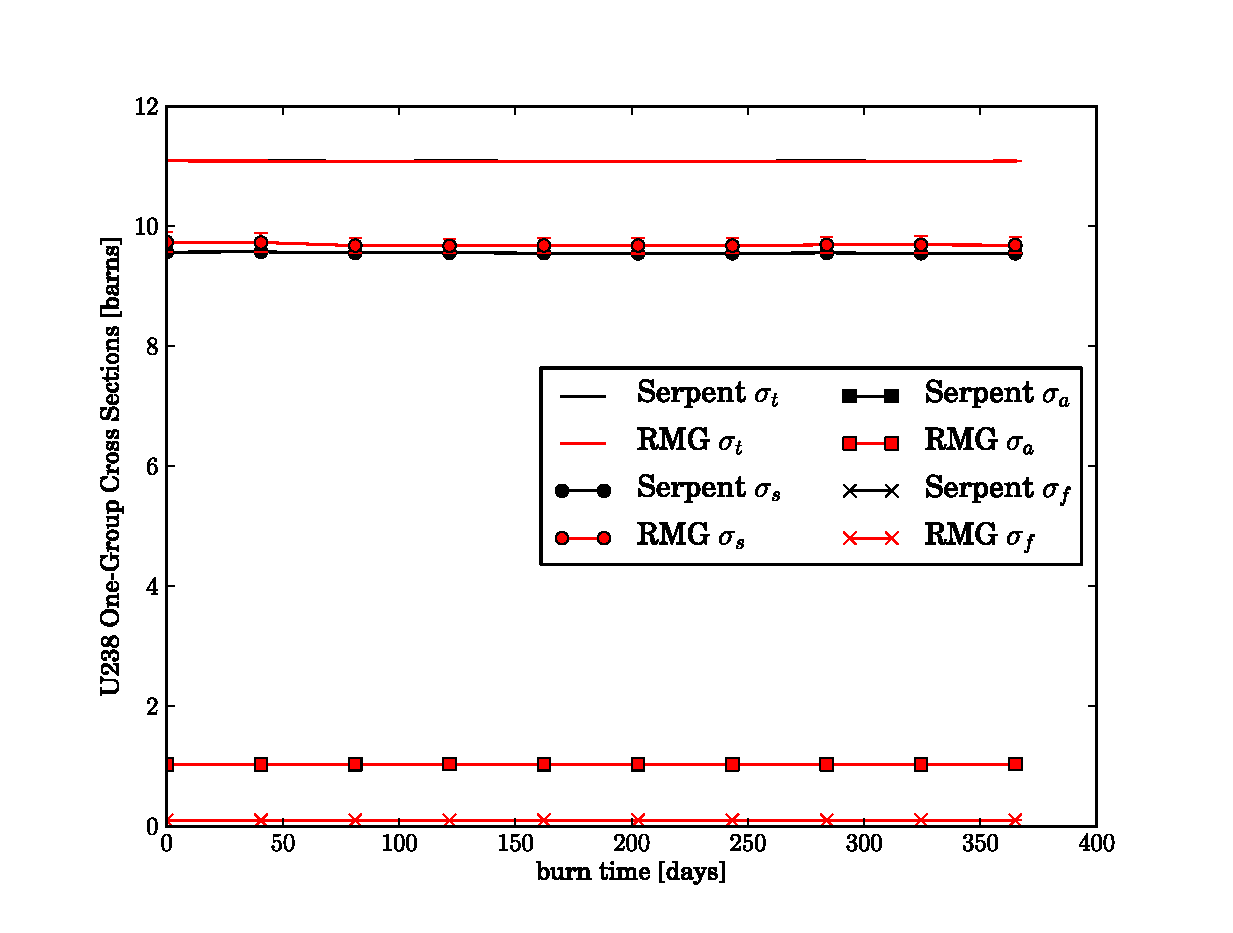
\includegraphics[scale=0.21]{../multigroup_method/figs/benchmark/U238_1g_xs.eps}}
\subfloat[\nuc{Pu}{239}]{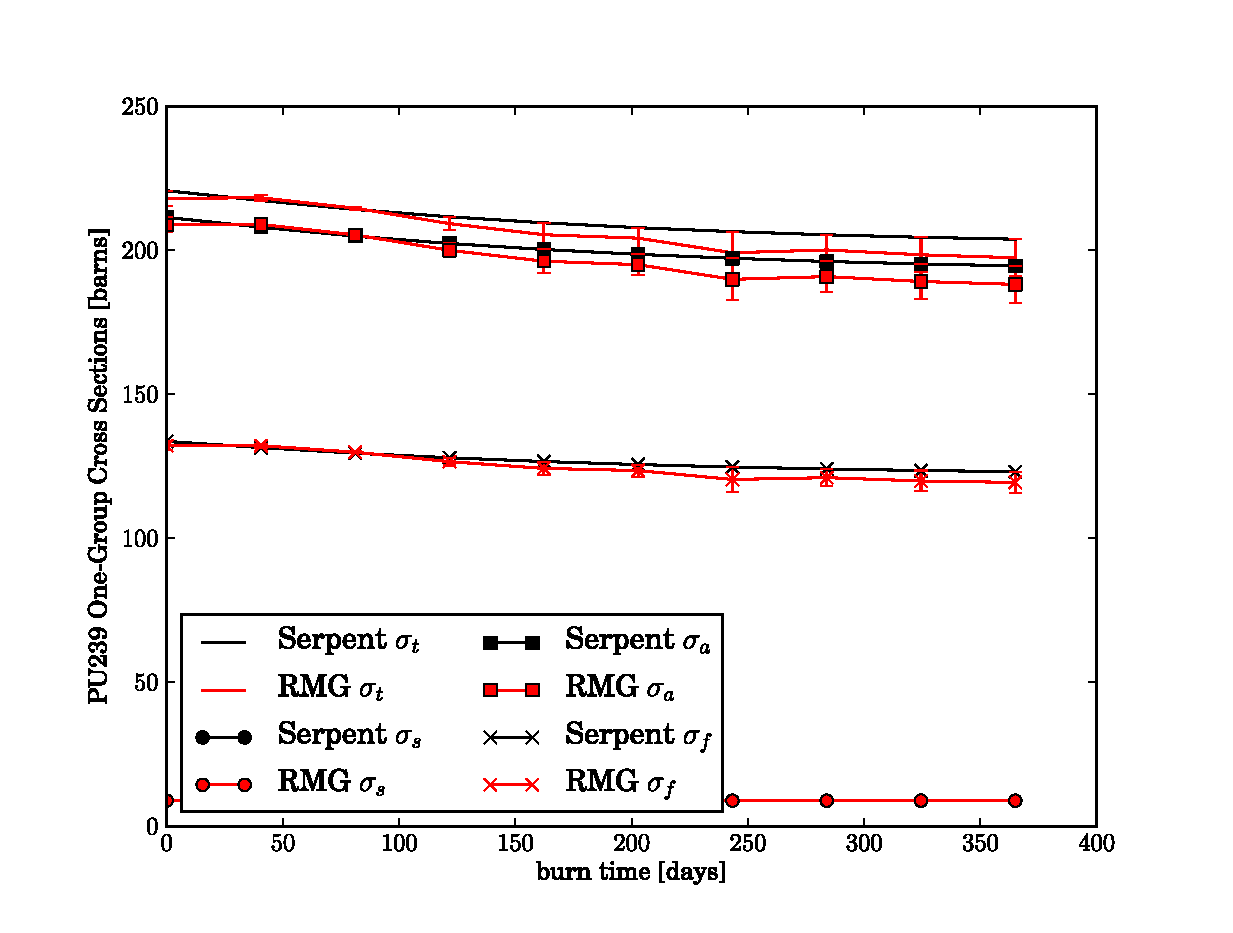
\includegraphics[scale=0.21]{../multigroup_method/figs/benchmark/PU239_1g_xs.eps}}
\end{figure}
\end{center}
\end{slide}




% RMG Benchmark
\begin{slide}{RMG Benchmark}
\vspace{0.75cm}
\begin{center}
\begin{figure}
\caption{Selected Actinide One-Group Cross-Sections}
\subfloat[\nuc{Pu}{240}]{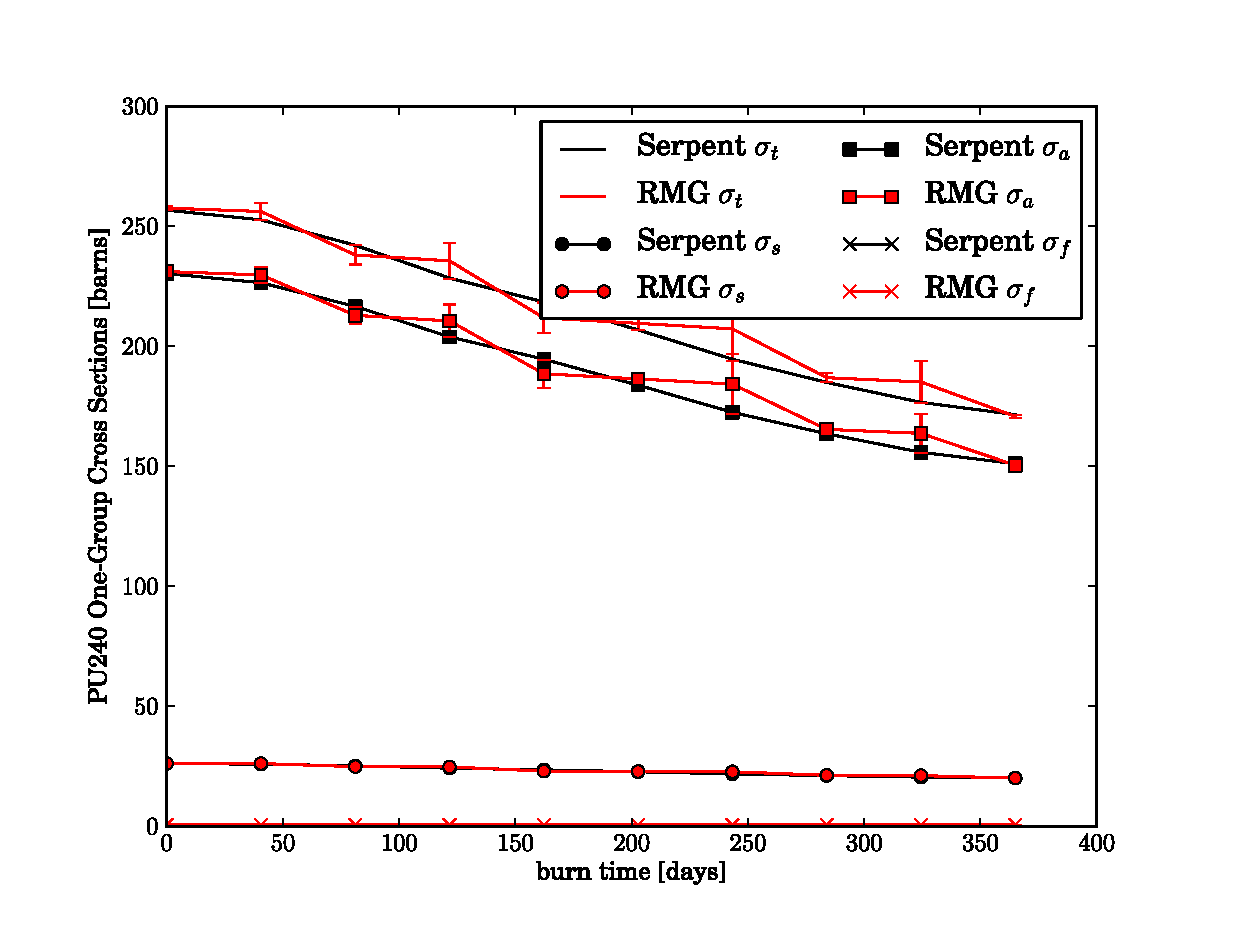
\includegraphics[scale=0.21]{../multigroup_method/figs/benchmark/PU240_1g_xs.eps}}
\subfloat[\nuc{Am}{242}]{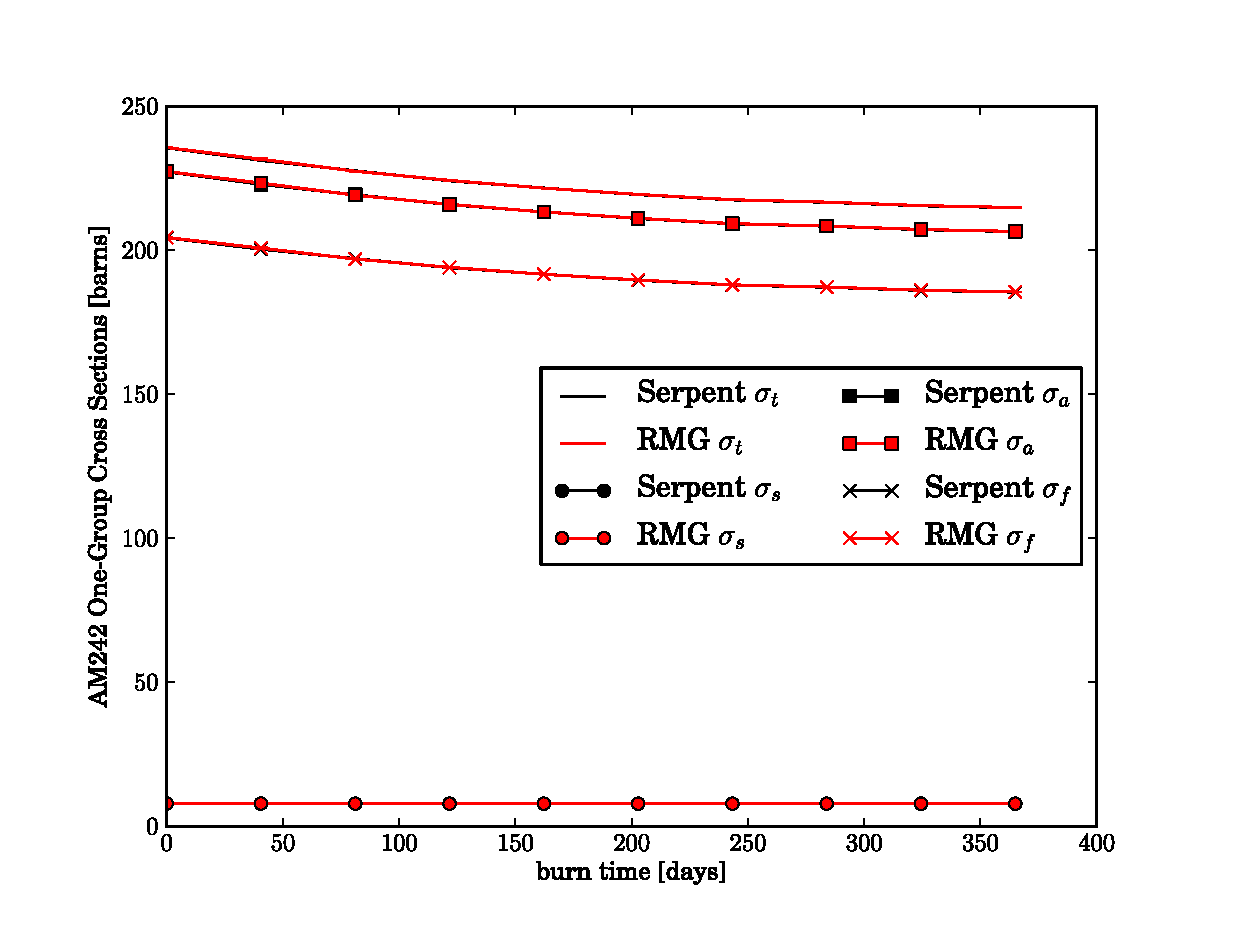
\includegraphics[scale=0.21]{../multigroup_method/figs/benchmark/AM242_1g_xs.eps}}
\subfloat[\nuc{Cm}{246}]{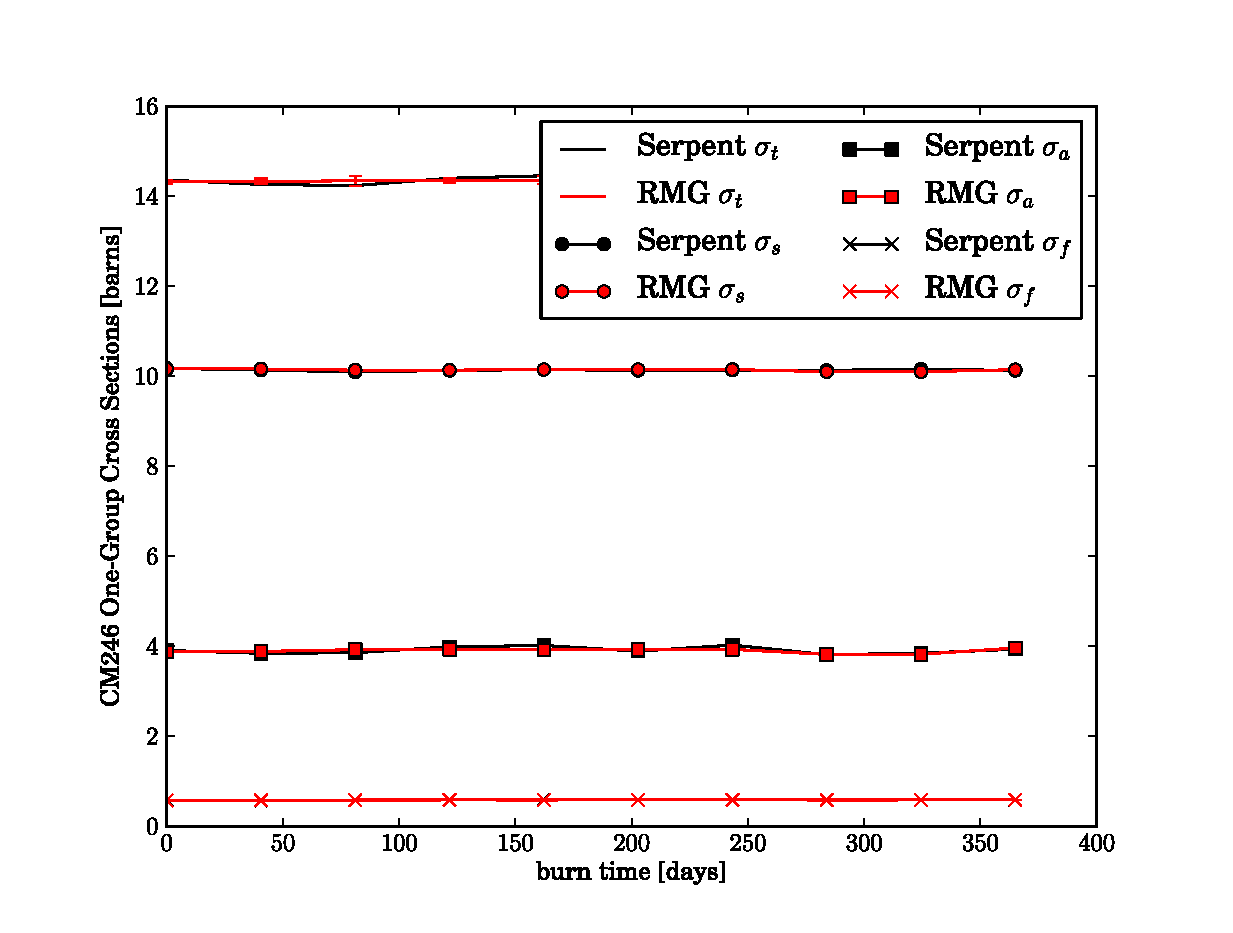
\includegraphics[scale=0.21]{../multigroup_method/figs/benchmark/CM246_1g_xs.eps}}
\end{figure}
\end{center}
\end{slide}



% RMG Benchmark
\begin{slide}{RMG Benchmark}
\vspace{0.75cm}
\begin{center}
\begin{figure}
\caption{Fission Product One-Group Cross-Sections}
\subfloat[\nuc{Sr}{90}]{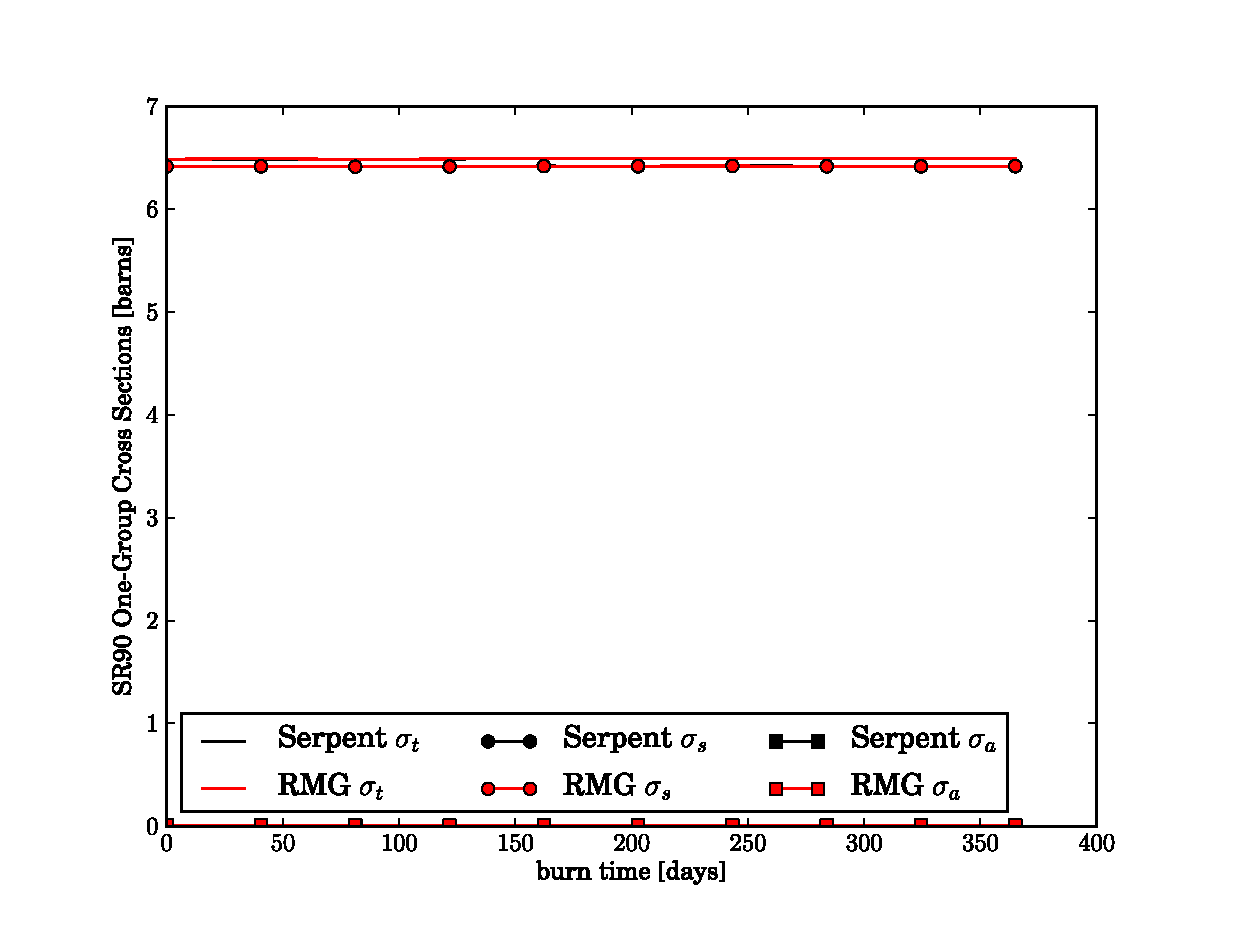
\includegraphics[scale=0.21]{../multigroup_method/figs/benchmark/SR90_1g_xs.eps}}
\subfloat[\nuc{Tc}{99}]{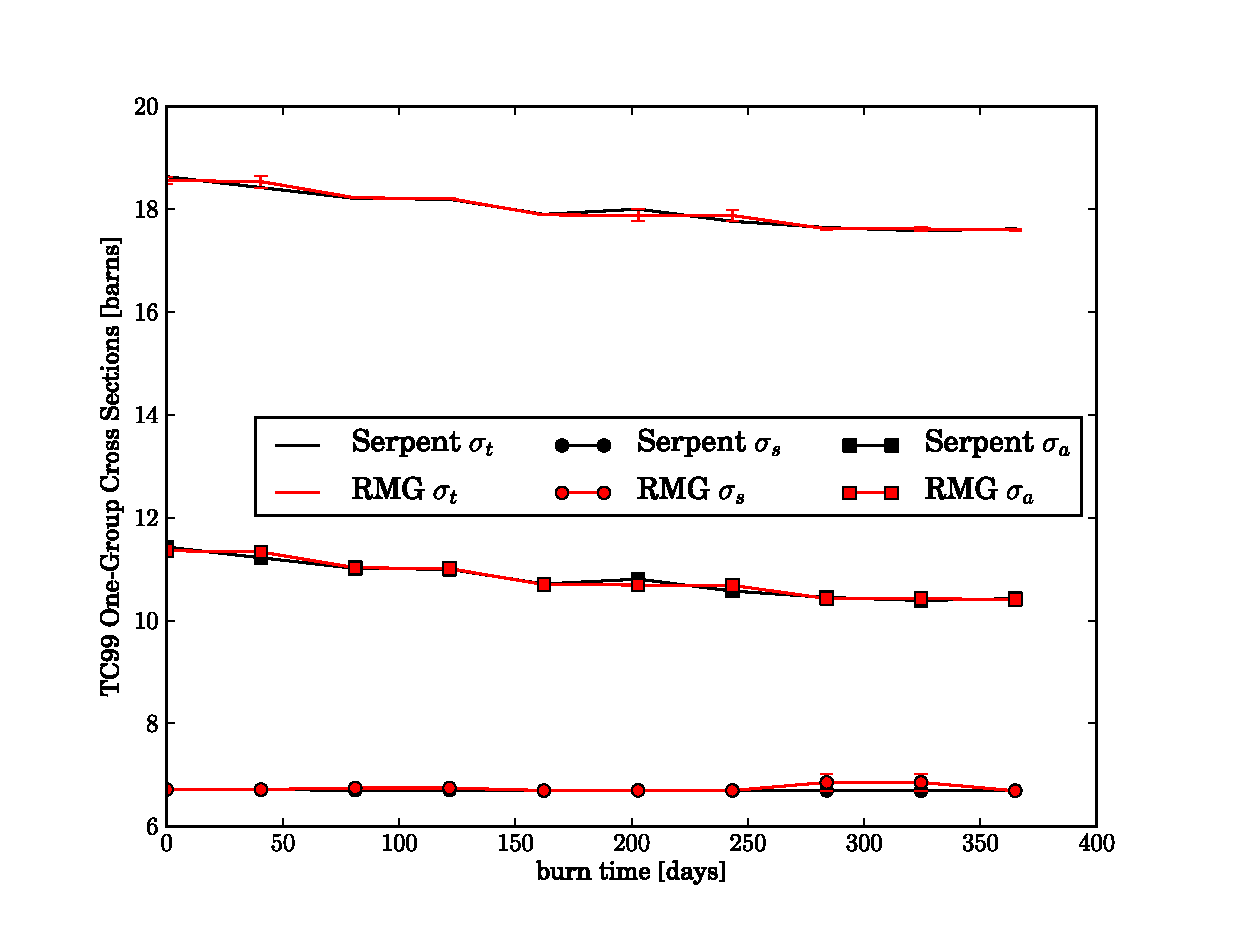
\includegraphics[scale=0.21]{../multigroup_method/figs/benchmark/TC99_1g_xs.eps}}
\subfloat[\nuc{Cs}{137}]{\includegraphics[scale=0.21]{../multigroup_method/figs/benchmark/CS137_1g_xs.eps}}
\end{figure}
\end{center}
\end{slide}










%
% OMG next section
%

% Fuel Cycle Definition \& Benchmark
\begin{slide}{Definition \& Benchmark}
\vspace{3.5cm}
\begin{center}
\Large
Fuel Cycle Definition \& Benchmark
\end{center}
\end{slide}











% Fuel Cycle
\overlays{2}{
\begin{slide}{Fuel Cycle}
\FromSlide{1}
\begin{itemize}
    \item The essential physics models from before were
        used it to study a Fast Reactor (FR), Light
        Water Reactor (LWR) symbiotic scenario 
        analogous to Scheme 3a of a 2006 OECD report [3].
\end{itemize}

\FromSlide{2}
\setcounter{figure}{15}
\begin{center}
\begin{figure}
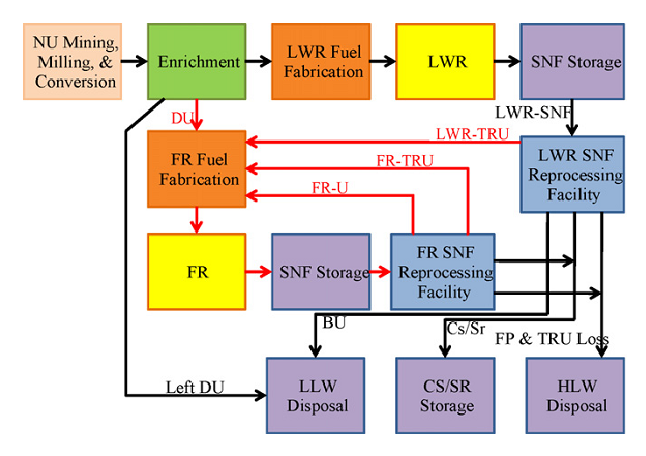
\includegraphics[scale=0.2]{../one_group_method/figs/Fig09.eps}
\caption{LWR-FR Fuel Cycle}
\end{figure}
\end{center}
\end{slide}}




% Fuel Cycle
\overlays{3}{
\begin{slide}{Fuel Cycle}
\FromSlide{1}
\small
With perturbable components, over 30 independent physical 
parameters may be adjusted in the fuel cycle.
\FromSlide{2}
\setcounter{figure}{16}
\begin{figure}
\begin{center}
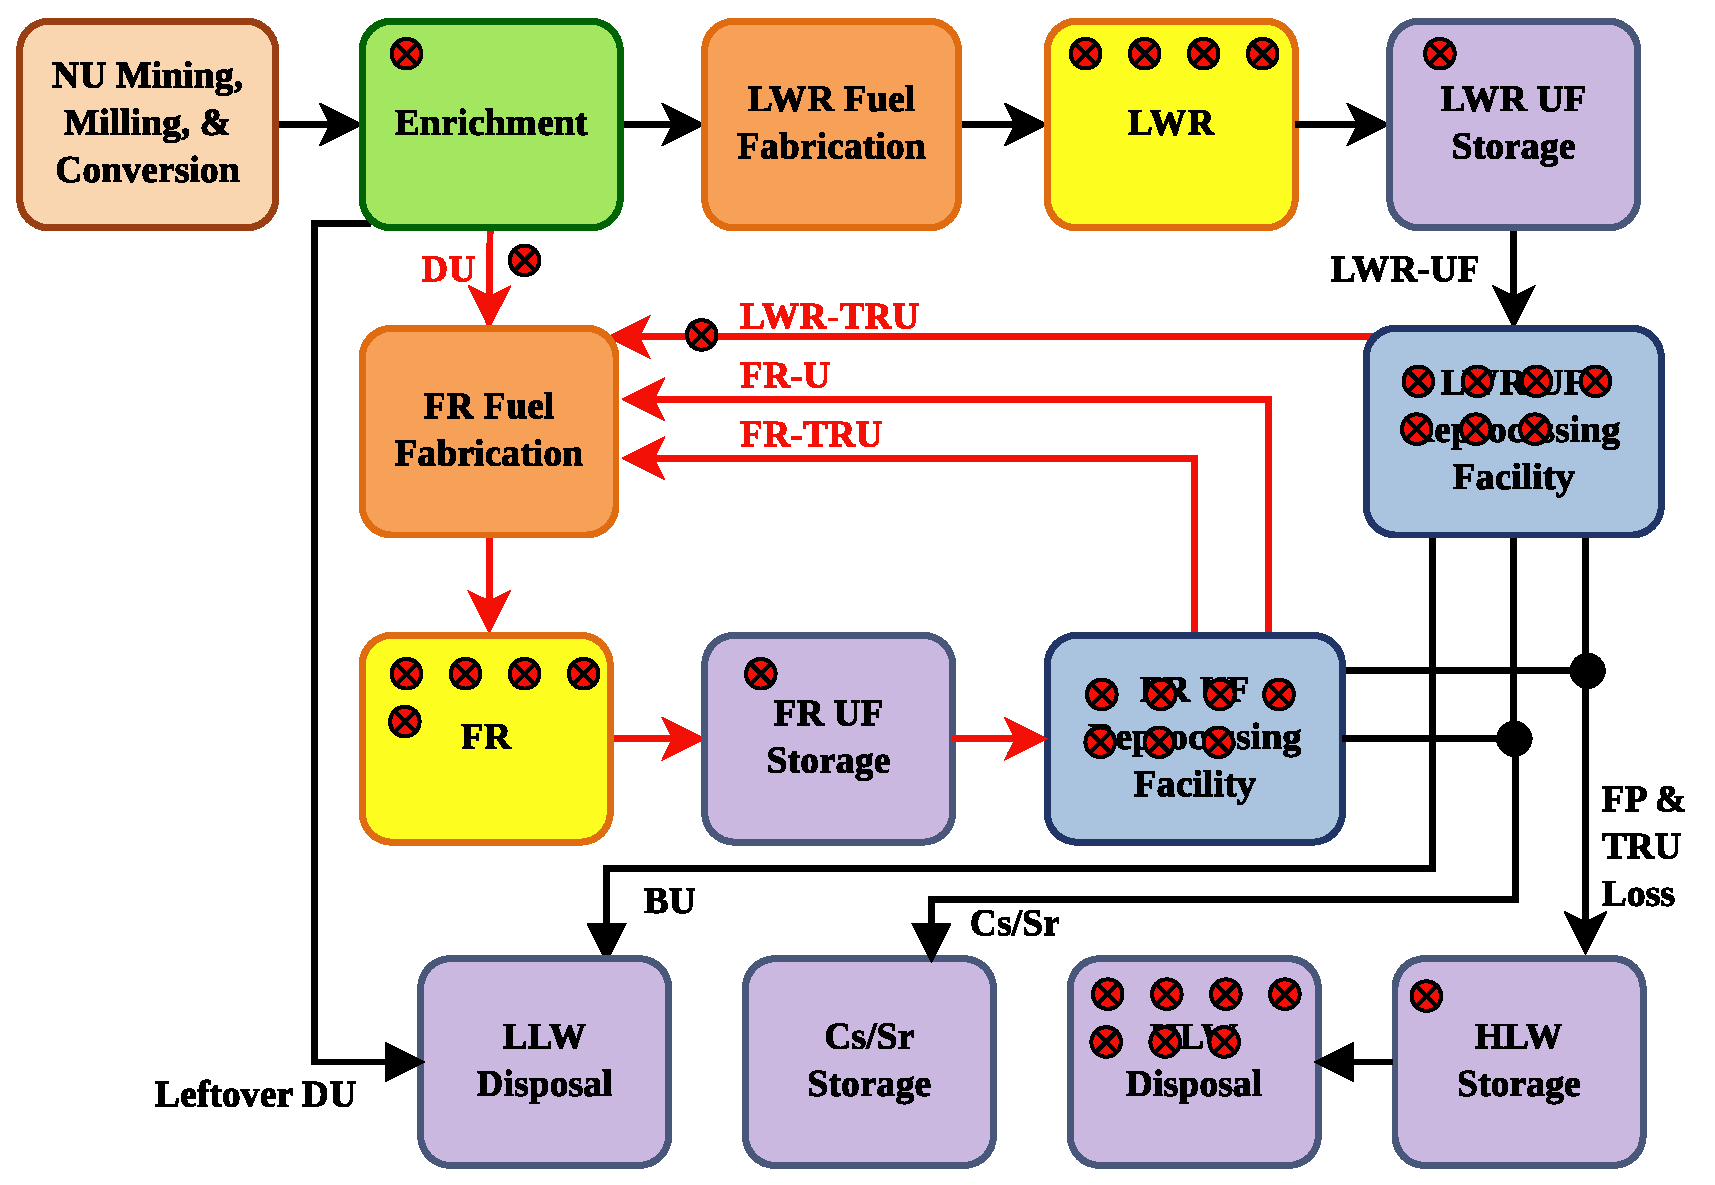
\includegraphics[scale=0.2]{figs/LWR_FR_FC_knobs.eps}
\caption{LWR-FR Cycle with Parameters}
\end{center}
\end{figure}
\FromSlide{3}
\small
Sensitivity results are computed from equilibrium values derived from 
a full treatment of the preceding, transient cycles.
\end{slide}}





% Fuel Cycle Benchmark
\begin{slide}{Fuel Cycle Base Case Benchmark}
\tiny
\begin{center}
\begin{tabular}{|l||c||c|c||c|c|}
\hline
\textbf{Scheme 3a}     & \textbf{NEA [3]} & \textbf{Model\superscript{1}} & \textbf{\% Diff} & \textbf{Model\superscript{2}} & \textbf{\% Diff} \\
\hline
Electricity Share: LWR & 0.632       & 0.619459             & -2.0244 & 0.634907             & +0.4579 \\
\hline
Electricity Share: FR  & 0.368       & 0.380541             & +3.2955 & 0.365093             & -0.7962 \\
\hline
FR UF: U               & 0.698       & 0.713806             & +2.2143 & 0.715224             & +2.4082 \\
\hline
FR UF: NP              & 0.0065      & 0.00661961           & +1.8070 & 0.00685174           & +5.1335 \\
\hline
FR UF: PU              & 0.266       & 0.248059             & -7.2327 & 0.248319             & -7.1204 \\
\hline
FR UF: AM              & 0.02        & 0.0226796            & 11.8152 & 0.0217317            & +7.9687 \\
\hline
FR UF: CM              & 0.0098      & 0.00883517           & -10.920 & 0.00787319           & -24.4730\\
\hline
HLW: U                 & 0.013324    & 0.0132681            & -0.4213 & 0.0134448            & +0.8984 \\
\hline
HLW: NP                & 2.26542E-05 & 2.4079E-05           & +5.9173 & 2.41083E-05          & +6.0316 \\
\hline
HLW: PU                & 0.000704797 & 0.000658893          & -6.9668 & 0.000632361          & -11.4548\\
\hline
HLW: AM                & 5.03426E-05 & 5.63068E-05          & 10.5923 & 5.12344E-05          & +1.7405 \\
\hline
HLW: CM                & 2.18151E-05 & 1.99031E-05          & -9.6068 & 1.67094E-05          & -30.5563\\
\hline
HLW: FP                & 0.985876    & 0.985973             & +0.0098 & 0.985831             & -0.0046 \\
\hline
\end{tabular}
\end{center}

1: Model with initial LWR \nuc{U}{235} enrichment of 4.2 w/o. 

2: Model with LWR discharge burnup of 50 MWd/kg.
\end{slide}









%
% OMG next section
%

% Information Theoretic Fuel Cycle Analysis
\begin{slide}{Contingency Tables}
\vspace{3.5cm}
\begin{center}
\Large
Information Theoretic Analysis
\end{center}
\end{slide}





% Fuel Cycle Methodology
\overlays{4}{
\begin{slide}{Contingency Table Methodology}
\FromSlide{1}
\begin{itemize}
    \item Here, the system-wide impact of physical parameter perturbations is quantified.

\FromSlide{2}
    \item This is done by performing \textbf{Contingency Table} analysis for each parameter
        to the \underline{repository} \underline{capacity} response.  

\FromSlide{3}
    \item Denote fuel cycle responses as $R$ [GWh] for $x$ \& $y$ input parameters.

\FromSlide{4}
    \item \textbf{\underline{Goal:}} Determine strength of \textit{association} 
        between inputs and pairs of inputs to the response in a manner that is independent to:
        \begin{itemize}
            \item the form of the response to the input $R(x)$,
            \item any base-case set of initial inputs.
        \end{itemize}

\FromSlide{1}
\end{itemize}
\end{slide}}




% Fuel Cycle Methodology
\begin{slide}{Contingency Table Methodology}
\begin{center}
\begin{figure}
\caption{Monte Carlo Methodology \& Analysis}
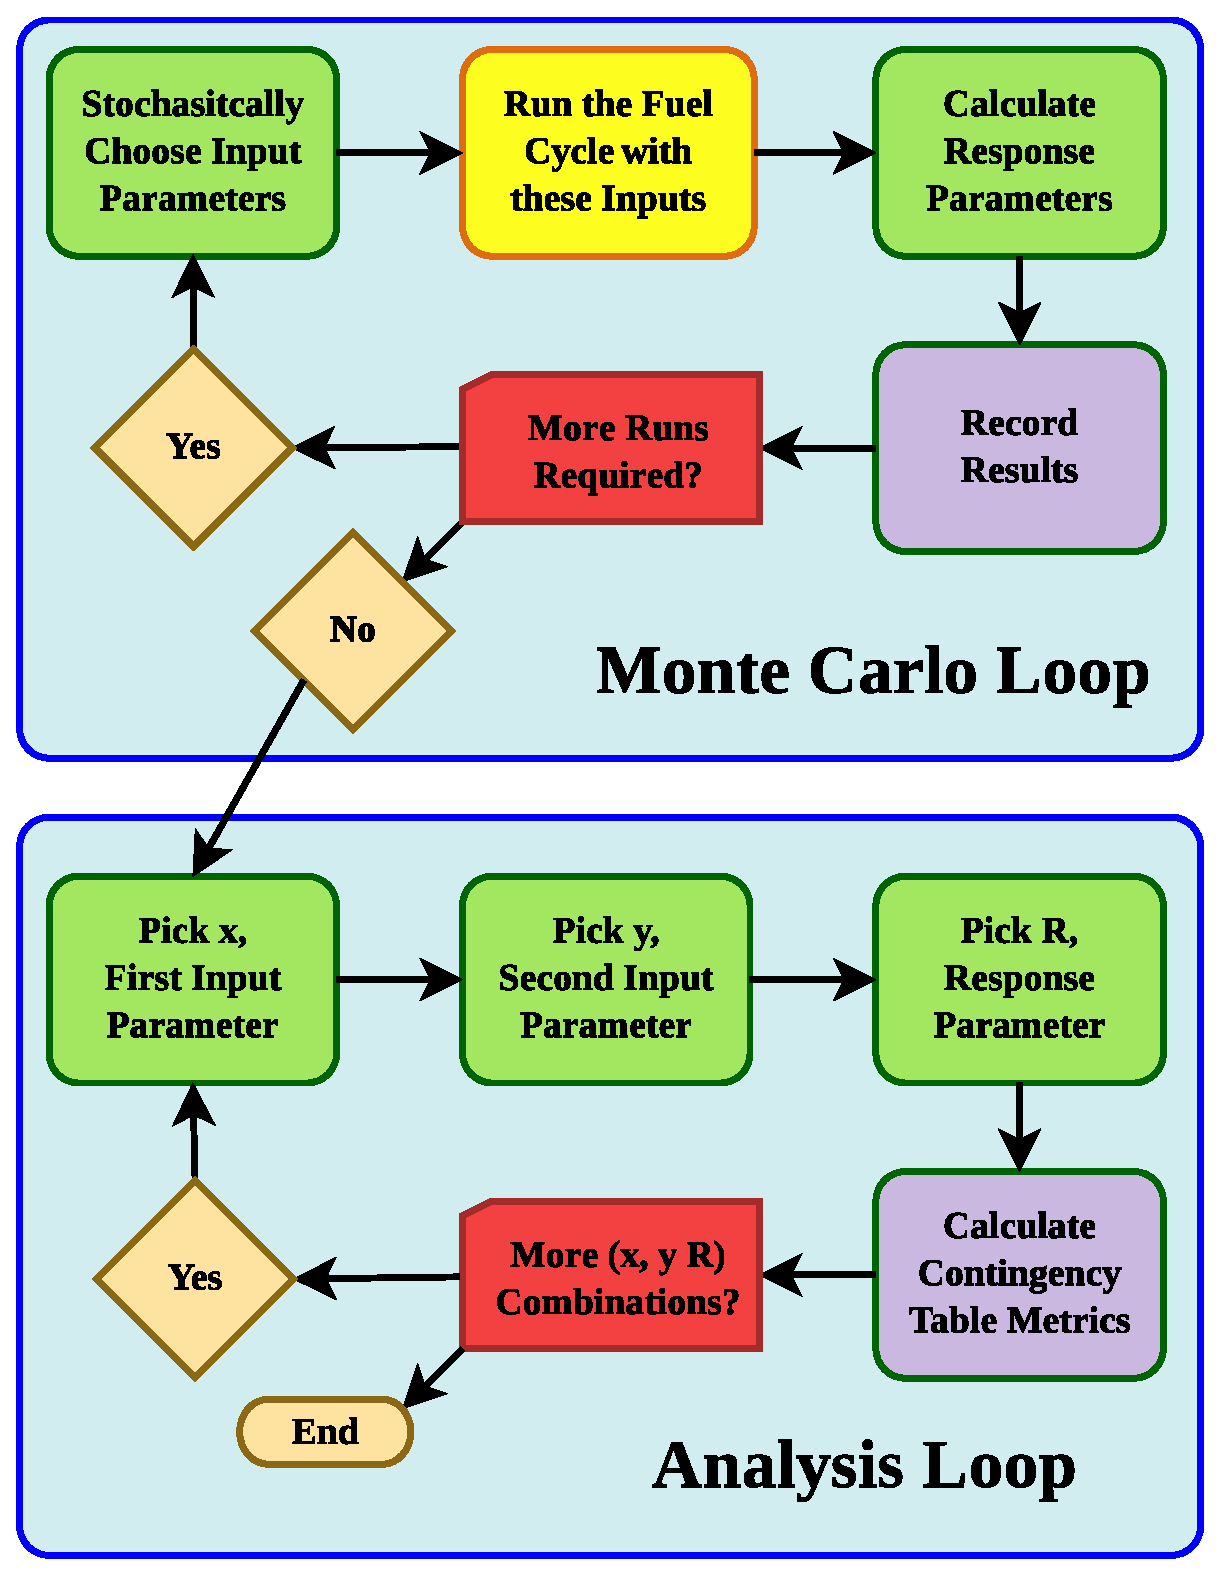
\includegraphics[scale=0.25]{../ct_sensitivity/figs/MonteCarloMethodology.eps}
\end{figure}
\end{center}
\end{slide}





% Input Parameter Definition
\begin{slide}{Input Parameter Definition}
\tiny
\begin{center}
\begin{tabular}{|l||c|c|c|c|}
\hline
\textbf{Input Parameter $x$} & \textbf{Min} & \textbf{Max} & \textbf{Units} & \textbf{Sample Type}\\
\hline
LWR Burnup Level & 30.0 & 80.0 & MWd/kgIHM & linear \\
\hline
LWR Fuel to Moderator Ratio & 0.28 & 0.36 & & linear \\
\hline
LWR SNF Storage Time & 3 & 30 & years & linear \\
\hline
SE of U from LWR UF & 0.99 & 0.9999 & & nines \\
\hline
SE of NP from LWR UF & 0.9 & 0.9999 & & nines \\
\hline
SE of PU from LWR UF & 0.9 & 0.9999 & & nines \\
\hline
SE of AM from LWR UF & 0.9 & 0.9999 & & nines \\
\hline
SE of CM from LWR UF & 0.9 & 0.9999 & & nines \\
\hline
SE of CS from LWR UF & 0.9 & 0.9999 & & nines \\
\hline
SE of SR from LWR UF & 0.9 & 0.9999 & & nines \\
\hline
FR Burnup Level & 100.0 & 200.0 & MWd/kgIHM & linear\\
\hline
FR TRU Conversion Ratio & 0.25 & 0.95 & & linear \\
\hline
Max Fraction of Lanthanide in FR Fuel & 0.0001 & 0.005 & Atoms/TRU Atom & linear \\
\hline
FR UF Storage Time & 3 & 30 & years & linear \\
\hline
Storage Before Disposal & 1 & 300 & years & log \\
\hline
\end{tabular}
\end{center}
\end{slide}

%Input Parameter Definition
\begin{slide}{Input Parameter Definition}
\tiny
\begin{center}
\begin{tabular}{|l||c|c|c|c|}
\hline
\textbf{Input Parameter $x$} & \textbf{Min} & \textbf{Max} & \textbf{Units} & \textbf{Sample Type}\\
\hline
SE of U from FR UF & 0.99 & 0.9999 & & nines \\
\hline
SE of NP from FR UF & 0.9 & 0.9999 & & nines \\
\hline
SE of PU from FR UF & 0.9 & 0.9999 & & nines \\
\hline
SE of AM from FR UF & 0.9 & 0.9999 & & nines \\
\hline
SE of CM from FR UF & 0.9 & 0.9999 & & nines \\
\hline
SE of CS from FR UF & 0.9 & 0.9999 & & nines \\
\hline
SE of SR from FR UF & 0.9 & 0.9999 & & nines \\
\hline
Density of Host Rock & 2317 & 2869 & kg/m\superscript{3} & linear \\
\hline
Specific Heat of Host Rock & 590 & 1270 & J/kg-K & linear \\
\hline
Thermal Conductivity of Host Rock & 1.9204 & 3.2856 & W/m-K & linear \\
\hline
Heat Loss Factor During Ventilation  & 0.806 & 0.914 & & linear \\
\hline
Drift diameter & 4.5 & 6.5 & m & linear \\
\hline
Ventilation System On Time & 10 & 300 & years & log \\
\hline
Ambient Environment Temperature & 12.82 & 32.82 & C & linear \\
\hline
Distance Between Drifts & 56 & 106 & m & linear \\
\hline
\end{tabular}
\end{center}
\end{slide}








% Contingency Tables
\overlays{3}{
\begin{slide}{Contingency Tables}
\FromSlide{1}
The $2\times 2$ table is most common:
\setcounter{table}{4}
\begin{center}
\begin{table}
\caption{Hair Color to Sex Contingency Table}
\begin{tabular}{|l||c|c||c|}
\hline
       & Blonde & Brunette & Totals \\
\hline
Female & 18     & 17       & 35 \\
\hline
Male   & 11     & 14       & 25 \\
\hline
Totals & 29     & 31       & 60 \\
\hline
\end{tabular}
\end{table}
\end{center} 

\FromSlide{2}
\vspace{0.5cm}
But doesn't this approach ignore the underlying biology?

\FromSlide{3}
\vspace{0.5cm}
\raggedleft{\LARGE \textit{Yes!}}
\end{slide}}



% Contingency Tables
\overlays{6}{
\begin{slide}{Contingency Tables}
\begin{center}
\onlySlide*{1}{
\includegraphics[scale=0.125]{figs/CTBlackBox/CTBlackBox01.eps}}

\onlySlide*{2}{
\includegraphics[scale=0.125]{figs/CTBlackBox/CTBlackBox02.eps}}

\onlySlide*{3}{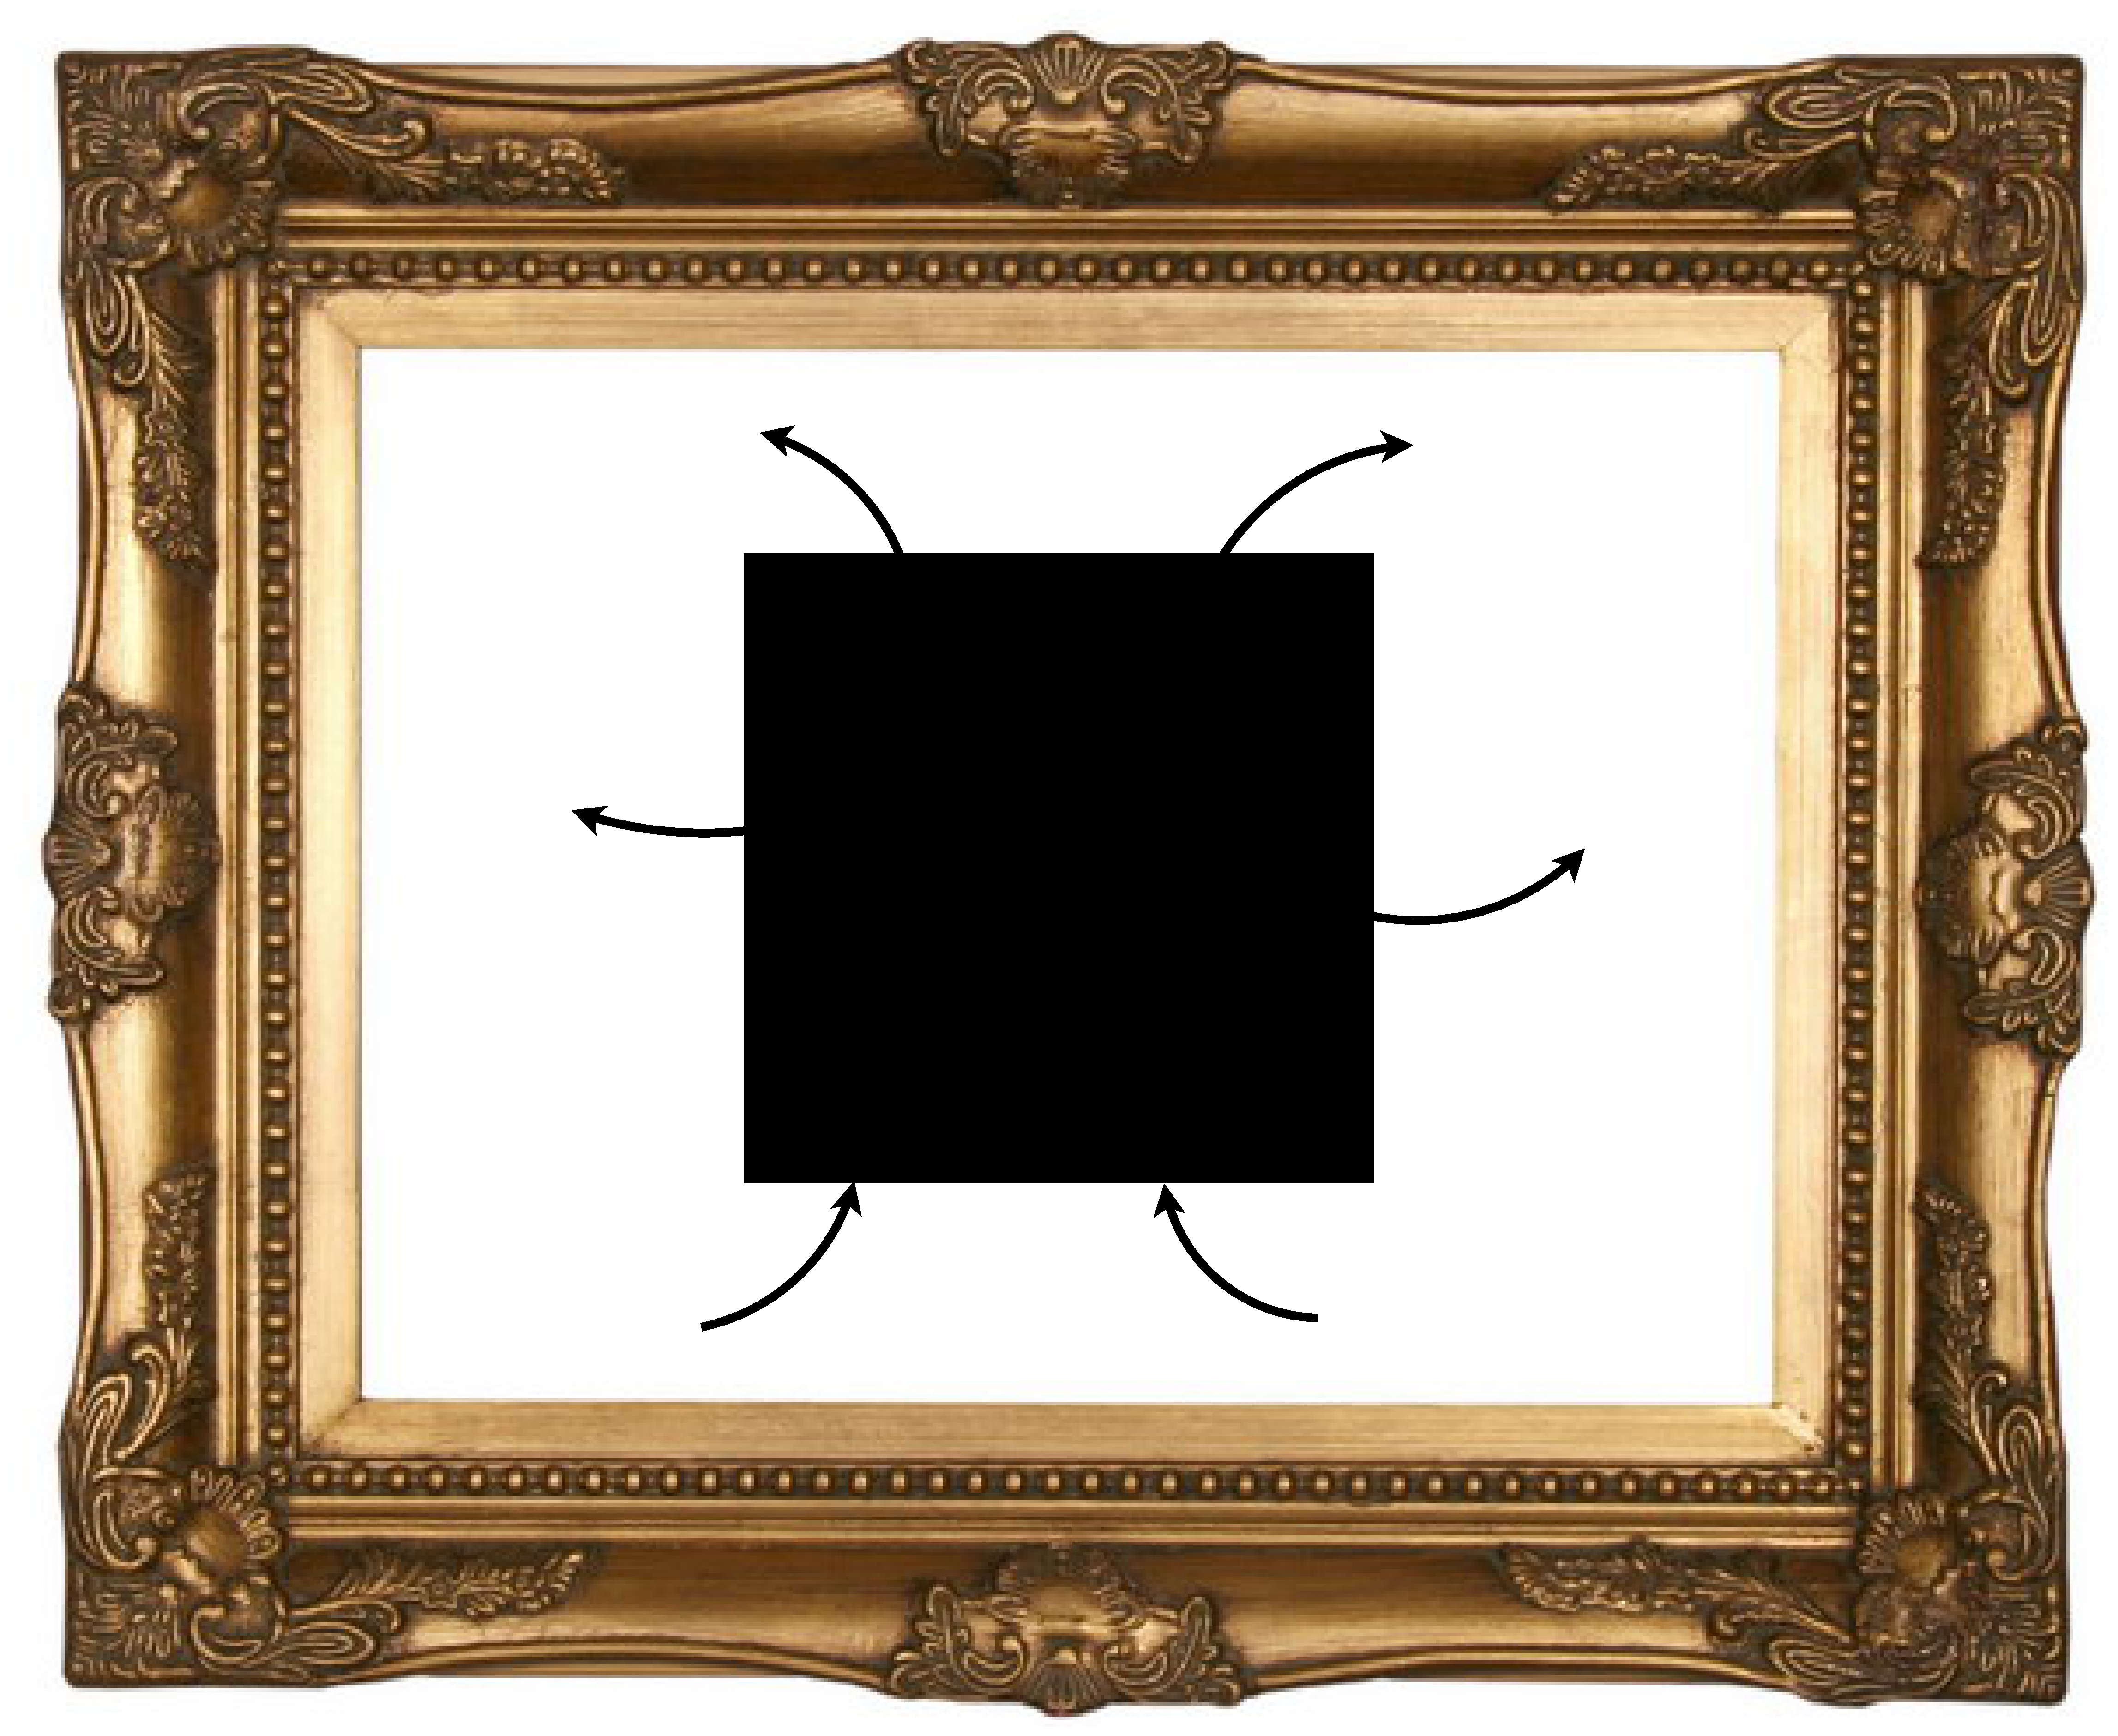
\includegraphics[scale=0.125]{figs/CTBlackBox/CTBlackBox03.eps}}

\onlySlide*{4}{
\includegraphics[scale=0.125]{figs/CTBlackBox/CTBlackBox04.eps}}

\onlySlide*{5}{
\includegraphics[scale=0.125]{figs/CTBlackBox/CTBlackBox05.eps}}

\onlySlide*{6}{
\includegraphics[scale=0.125]{figs/CTBlackBox/CTBlackBox06.eps}}
\end{center}
\end{slide}}



% Fuel Cycle Contingency Table
\overlays{2}{
\begin{slide}{Fuel Cycle Contingency Table}
\FromSlide{1}
For example, let's construct a 2D contingency table that 
measures the response from a sample input: fast reactor 
fuel plutonium separation efficiency, \texttt{FR\_SE\_PU}.

\FromSlide{2}
\vspace{0.50cm}
\begin{table}
\caption{Contingency Table for FR Plutonium SE to Repository Capacity [MTHM/Repository].}
\begin{center}
\footnotesize
\begin{tabular}{|c||c|c|c||c|}
\hline
&$0.9<$\texttt{SE}$<0.99$&$0.99<$\texttt{SE}$<0.999$&$0.999<$\texttt{SE}$<0.9999$&\\
\hline
$10^4 <$ \texttt{Capacity} $< 10^5$&$739$&$43$&$27$&$809$\\
\hline
$10^5 <$ \texttt{Capacity} $< 10^6$&$31510$&$21611$&$19469$&$72590$\\
\hline
$10^6 <$ \texttt{Capacity} $< 10^7$&$2648$&$13095$&$14430$&$30173$\\
\hline
$10^7 <$ \texttt{Capacity} $< 10^8$&$0$&$213$&$1053$&$1266$\\
\hline
&$34897$&$34962$&$34979$&$104838$\\
\hline
\end{tabular}
\end{center}
\label{ct2d_example}
\end{table}

\end{slide}}


% Contingency Table Statistics
\overlays{3}{
\begin{slide}{Contingency Table Statistics}
\FromSlide{1}
There are several metrics that have been developed to measure 
associations with contingency tables.  

\FromSlide{2}
\vspace{0.5cm}
The primary measure here is the \emph{Uncertainty Coefficient} $U(x|R)$.

\FromSlide{3}
\vspace{0.5cm}
To calculate $U(x|R)$ the following are needed, 
\begin{itemize}
    \item The \emph{Entropy} $H(x)$, which is a measure of how evenly the 
        data is spread out in the $x$ parameter.
    \item The \emph{Mutual Information} $I(R,x)$ which states the shared
        value of the $x$ together with $R$. 
\end{itemize}
\end{slide}}



% Contingency Table Statistics
\overlays{2}{
\begin{slide}{Contingency Table Statistics}
\FromSlide{1}
The uncertainty coefficient is then calculated from,
\[ U(x|R) = \frac{I(R,x)}{H(x)} \]

\FromSlide{2}
This metric has the following useful properties:
\begin{enumerate}
    \item Defined on the range $[0, 1]$.
    \item $U(x|R) = 0$ implies that $I(R,x) = 0$, which indicates that the parameter
        is unassociated with the response.
    \item $U(x|R) = 1$ requires that $I(R,x) = H(x)$.  This implies that
        the system response $R(x)$ is solely determined by $x$.
\end{enumerate}
\end{slide}}



% Input Parameters Ranked by $U(x|R)$
\begin{slide}{Input Parameters Ranked by $U(x|R)$}
\begin{center}
\tiny
\begin{tabular}{|r|l|c|}
\hline
\textbf{Rank} & \textbf{$x$} & \textbf{$U(x|R)$}\\
\hline
1&\texttt{FR\_SE\_PU}&0.07667\\
\hline
2&\texttt{HLW\_Storage\_Time}&0.05264\\
\hline
3&\texttt{FR\_SE\_AM}&0.04148\\
\hline
4&\texttt{Heat\_Loss\_Factor}&0.01548\\
\hline
5&\texttt{LWR\_SE\_PU}&0.01343\\
\hline
6&\texttt{FR\_TRU\_CR}&0.008895\\
\hline
7&\texttt{LWR\_SE\_AM}&0.007304\\
\hline
8&\texttt{FR\_BUd}&0.003773\\
\hline
9&\texttt{LWR\_UF\_Storage\_Time}&0.003551\\
\hline
10&\texttt{Rock\_Specific\_Heat}&0.003085\\
\hline
11&\texttt{FR\_SE\_CM}&0.002522\\
\hline
12&\texttt{Rock\_Thermal\_Conductivity}&0.001954\\
\hline
13&\texttt{Ambient\_Temp}&0.001353\\
\hline
14&\texttt{LWR\_BUd}&0.001053\\
\hline
15&\texttt{LWR\_SE\_CS}&0.001033\\
\hline
\end{tabular}
\end{center}
\end{slide}



% Input Parameters Ranked by $U(x|R)$
\begin{slide}{Input Parameters Ranked by $U(x|R)$}
\begin{center}
\tiny
\begin{tabular}{|r|l|c|}
\hline
\textbf{Rank} & \textbf{$x$} & \textbf{$U(x|R)$}\\
\hline
16&\texttt{LWR\_SE\_SR}&0.001024\\
\hline
17&\texttt{FR\_UF\_Storage\_Time}&0.0005559\\
\hline
18&\texttt{Drift\_Space}&0.0004421\\
\hline
19&\texttt{LWR\_SE\_U}&0.0002899\\
\hline
20&\texttt{Rock\_Density}&0.0002718\\
\hline
21&\texttt{FR\_SE\_CS}&0.0001331\\
\hline
22&\texttt{FR\_SE\_SR}&0.0001073\\
\hline
23&\texttt{Vent\_System\_On\_Time}&0.0001016\\
\hline
24&\texttt{Drift\_Diameter}&9.648E-05\\
\hline
25&\texttt{LWR\_SE\_NP}&9.575E-05\\
\hline
26&\texttt{LWR\_SE\_CM}&7.969E-05\\
\hline
27&\texttt{LWR\_Fuel2Mod}&7.833E-05\\
\hline
28&\texttt{FR\_LAN\_FF\_Cap}&6.559E-05\\
\hline
29&\texttt{FR\_SE\_NP}&6.212E-05\\
\hline
30&\texttt{FR\_SE\_U}&6.207E-05\\
\hline
\end{tabular}
\end{center}
\end{slide}
















% Conclusions
\overlays{6}{
\begin{slide}{Conclusions}
\FromSlide{1}
\begin{itemize}
    \item Previous NFC simulators are either: 

    \FromSlide{2}
    \begin{itemize}
        \item not physics-based models, or

    \FromSlide{3}
        \item have prohibitively long run times.

    \FromSlide{2}
    \end{itemize}

\FromSlide{4}
    \vspace{0.3cm}
    \item Because of these limitations, only static base cases and linear 
        sensitivity analyses have historically been considered. 

\FromSlide{5}
    \vspace{0.3cm}
    \item Therefore large gaps in the analysis space existed. 

\FromSlide{6}
    \vspace{0.3cm}
    \item The essential physics models presented here effectively and efficiently address such limitations.

\FromSlide{1}
\end{itemize}
\end{slide}}







% Conclusions
\overlays{3}{
\begin{slide}{Conclusions}
\FromSlide{1}
\begin{itemize}
    \item The modeling suite presented here is a new, multi-scale approach to fuel cycle system design.

\FromSlide{2}
    \vspace{1.25cm}
    \item In fact, the speed and fidelity at which the underlying models operate \emph{enables} the new 
        fuel cycle analytics which were demonstrated.

\FromSlide{3}
    \vspace{1.25cm}
    \item It is now possible to tightly couple engineering concerns from multiple components simultaneously. 

\FromSlide{1}
\end{itemize}
\end{slide}}






% Proposed Future Work
\overlays{5}{
\begin{slide}{Proposed Future Work}
\FromSlide{1}
\begin{itemize}
    \item Fuel Cycle / Performance Assessment Simulator (GUI).

\FromSlide{2}
    \vspace{0.3cm}
    \item PyNE, a general purpose nuclear development environment.

\FromSlide{3}
    \vspace{0.3cm}
    \item Optimizations and improvements to the RMG.

\FromSlide{4}
    \vspace{0.3cm}
    \item Tighter integration with the repository model.

\FromSlide{5}
    \vspace{0.3cm}
    \item Categorical fuel cycle analysis.

\FromSlide{1}
\end{itemize}
\end{slide}}








% Questions
\begin{slide}{Questions}
? ? ? ? ? ? ? ? ? ? ? ? ? ? ? ? ? ? ? ? ? ? ? ? ? ? ? ? ? ? ? 
? ? ? ? ? ? ? ? ? ? ? ? ? ? ? ? ? ? ? ? ? ? ? ? ? ? ? ? ? ? ? 
? ? ? ? ? ? ? ? ? ? ? ? ? ? ? ? ? ? ? ? ? ? ? ? ? ? ? ? ? ? ? 
? ? ? ? ? ? ? ? ? ? ? ? ? ? ? ? ? ? ? ? ? ? ? ? ? ? ? ? ? ? ? 
? ? ? ? ? ? ? ? ? ? ? ? ? ? ? ? ? ? ? ? ? ? ? ? ? ? ? ? ? ? ? 
? ? ? ? ? ? ? ? ? ? ? ? ? ? ? ? ? ? ? ? ? ? ? ? ? ? ? ? ? ? ? 
? ? ? ? ? ? ? ? ? ? ? ? ? ? ? ? ? ? ? ? ? ? ? ? ? ? ? ? ? ? ? 
? ? ? ? ? ? ? ? ? ? ? ? ? ? ? ? ? ? ? ? ? ? ? ? ? ? ? ? ? ? ? 
? ? ? ? ? ? ? ? ? ? ? ? ? ? ? ? ? ? ? ? ? ? ? ? ? ? ? ? ? ? ? 
? ? ? ? ? ? ? ? ? ? ? ? ? ? ? ? ? ? ? ? ? ? ? ? ? ? ? ? ? ? ? 
? ? ? ? ? ? ? ? ? ? ? ? ? ? ? ? ? ? ? ? ? ? ? ? ? ? ? ? ? ? ? 
? ? ? ? ? ? ? ? ? ? ? ? ? ? ? ? ? ? ? ? ? ? ? ? ? ? ? ? ? ? ? 
? ? ? ? ? ? ? ? ? ? ? ? ? ? ? ? ? ?
\end{slide}

\begin{slide}{Bibliography}
\tiny
\begin{enumerate}
    \item \fullcite{Scopatz2009}
    \item \fullcite{Takano1994}
    \item \fullcite{NEA-5990}
    \item \fullcite{Press2007c}
    \item \fullcite{ENDF}
    \item \fullcite{Lepp2011}
    \item \fullcite{Croff2002}
\end{enumerate}
\end{slide}

\end{document}
